%-----------------------------------------------------------------------------------------
% Autor dieser Vorlage:
% Stefan Macke (http://fachinformatiker-anwendungsentwicklung.net)
% Permalink zur Vorlage: http://fiae.link/LaTeXVorlageFIAE
%
% Sämtliche verwendeten Abbildungen, Tabellen und Listings stammen von Dirk Grashorn.
%
% Lizenz: Creative Commons 4.0 Namensnennung - Weitergabe unter gleichen Bedingungen
% -----------------------------------------------------------------------------------------

\documentclass[
	ngerman,
	toc=listof, % Abbildungsverzeichnis sowie Tabellenverzeichnis in das Inhaltsverzeichnis aufnehmen
	toc=bibliography, % Literaturverzeichnis in das Inhaltsverzeichnis aufnehmen
	footnotes=multiple, % Trennen von direkt aufeinander folgenden Fußnoten
	parskip=half, % vertikalen Abstand zwischen Absätzen verwenden anstatt horizontale Einrückung von Folgeabsätzen
	numbers=noendperiod % Den letzten Punkt nach einer Nummerierung entfernen (nach DIN 5008)
, 11pt]{scrartcl}
\pdfminorversion=5 % erlaubt das Einfügen von pdf-Dateien bis Version 1.7, ohne eine Fehlermeldung zu werfen (keine Garantie für fehlerfreies Einbetten!)
\usepackage[utf8]{inputenc} % muss als erstes eingebunden werden, da Meta/Packages ggfs. Sonderzeichen enthalten

%\usepackage{booktabs}

% !TEX root = Projektdokumentation.tex

% Hinweis: der Titel muss zum Inhalt des Projekts passen und den zentralen Inhalt des Projekts deutlich herausstellen
\newcommand{\titel}{Entwicklung einer Statistik-App}
\newcommand{\untertitel}{Webbasierte App zur statistischen Analyse von KPIs}
\newcommand{\kompletterTitel}{\titel{} -- \untertitel}

\newcommand{\autorName}{Steven Hergt}
\newcommand{\autorAnschrift}{Georg-Büchner-Str. 9}
\newcommand{\autorOrt}{07749 Jena}

\newcommand{\betriebLogo}{logo_164px.png}
\newcommand{\betriebName}{ePages GmbH}
\newcommand{\betriebAnschrift}{Heinrich-Heine-Str. 1}
\newcommand{\betriebOrt}{07749 Jena}

\newcommand{\ausbildungsberuf}{Fachinformatiker für Anwendungsentwicklung}
\newcommand{\betreff}{Dokumentation zur betrieblichen Projektarbeit}
\newcommand{\pruefungstermin}{Winter 2016/17}
\newcommand{\abgabeOrt}{Gera}
\newcommand{\abgabeTermin}{30.11.2016}
 % Metadaten zu diesem Dokument (Autor usw.)
% !TEX root = ../Projektdokumentation.tex

% Anpassung an Landessprache ---------------------------------------------------
\usepackage{babel}

% Umlaute ----------------------------------------------------------------------
%   Umlaute/Sonderzeichen wie äüöß direkt im Quelltext verwenden (CodePage).
%   Erlaubt automatische Trennung von Worten mit Umlauten.
% ------------------------------------------------------------------------------
\usepackage[T1]{fontenc}
\usepackage{textcomp} % Euro-Zeichen etc.

% Schrift ----------------------------------------------------------------------
\usepackage{lmodern} % bessere Fonts
\usepackage{relsize} % Schriftgröße relativ festlegen

% Tabellen ---------------------------------------------------------------------
\PassOptionsToPackage{table}{xcolor}
\usepackage{tabularx}
% für lange Tabellen
\usepackage{longtable}
\usepackage{array}
\usepackage{ragged2e}
\usepackage{lscape}
\newcolumntype{w}[1]{>{\raggedleft\hspace{0pt}}p{#1}} % Spaltendefinition rechtsbündig mit definierter Breite

% Grafiken ---------------------------------------------------------------------
\usepackage[dvips,final]{graphicx} % Einbinden von JPG-Grafiken ermöglichen
\usepackage{graphics} % keepaspectratio
\usepackage{floatflt} % zum Umfließen von Bildern
\graphicspath{{Bilder/}} % hier liegen die Bilder des Dokuments

% Sonstiges --------------------------------------------------------------------
\usepackage[titles]{tocloft} % Inhaltsverzeichnis DIN 5008 gerecht einrücken
\usepackage{amsmath,amsfonts} % Befehle aus AMSTeX für mathematische Symbole
\usepackage{enumitem} % anpassbare Enumerates/Itemizes
\usepackage{xspace} % sorgt dafür, dass Leerzeichen hinter parameterlosen Makros nicht als Makroendezeichen interpretiert werden

\usepackage{makeidx} % für Index-Ausgabe mit \printindex
\usepackage[printonlyused]{acronym} % es werden nur benutzte Definitionen aufgelistet

% Einfache Definition der Zeilenabstände und Seitenränder etc.
\usepackage{setspace}
\usepackage{geometry}

% Symbolverzeichnis
\usepackage[intoc]{nomencl}
\let\abbrev\nomenclature
\renewcommand{\nomname}{Abkürzungsverzeichnis}
\setlength{\nomlabelwidth}{.25\hsize}
\renewcommand{\nomlabel}[1]{#1 \dotfill}
\setlength{\nomitemsep}{-\parsep}

\usepackage{varioref} % Elegantere Verweise. „auf der nächsten Seite“
\usepackage{url} % URL verlinken, lange URLs umbrechen etc.

\usepackage{chngcntr} % fortlaufendes Durchnummerieren der Fußnoten
% \usepackage[perpage]{footmisc} % Alternative: Nummerierung der Fußnoten auf jeder Seite neu

\usepackage{ifthen} % bei der Definition eigener Befehle benötigt
\usepackage{todonotes} % definiert u.a. die Befehle \todo und \listoftodos
\usepackage[square]{natbib} % wichtig für korrekte Zitierweise

% PDF-Optionen -----------------------------------------------------------------
\usepackage{pdfpages}
\pdfminorversion=5 % erlaubt das Einfügen von pdf-Dateien bis Version 1.7, ohne eine Fehlermeldung zu werfen (keine Garantie für fehlerfreies Einbetten!)
\usepackage[
    bookmarks,
    bookmarksnumbered,
    bookmarksopen=true,
    bookmarksopenlevel=1,
    colorlinks=true,
% diese Farbdefinitionen zeichnen Links im PDF farblich aus
    linkcolor=AOBlau, % einfache interne Verknüpfungen
    anchorcolor=AOBlau,% Ankertext
    citecolor=AOBlau, % Verweise auf Literaturverzeichniseinträge im Text
    filecolor=AOBlau, % Verknüpfungen, die lokale Dateien öffnen
    menucolor=AOBlau, % Acrobat-Menüpunkte
    urlcolor=AOBlau,
% diese Farbdefinitionen sollten für den Druck verwendet werden (alles schwarz)
    %linkcolor=black, % einfache interne Verknüpfungen
    %anchorcolor=black, % Ankertext
    %citecolor=black, % Verweise auf Literaturverzeichniseinträge im Text
    %filecolor=black, % Verknüpfungen, die lokale Dateien öffnen
    %menucolor=black, % Acrobat-Menüpunkte
    %urlcolor=black,
%
    %backref, % Quellen werden zurück auf ihre Zitate verlinkt
    pdftex,
    plainpages=false, % zur korrekten Erstellung der Bookmarks
    pdfpagelabels=true, % zur korrekten Erstellung der Bookmarks
    hypertexnames=false, % zur korrekten Erstellung der Bookmarks
    linktocpage % Seitenzahlen anstatt Text im Inhaltsverzeichnis verlinken
]{hyperref}
% Befehle, die Umlaute ausgeben, führen zu Fehlern, wenn sie hyperref als Optionen übergeben werden
\hypersetup{
    pdftitle={\titel -- \untertitel},
    pdfauthor={\autorName},
    pdfcreator={\autorName},
    pdfsubject={\titel -- \untertitel},
    pdfkeywords={\titel -- \untertitel},
}


% zum Einbinden von Programmcode -----------------------------------------------
\usepackage{listings}
\usepackage{xcolor}
\definecolor{hellgelb}{rgb}{1,1,0.9}
\definecolor{colKeys}{rgb}{0,0,1}
\definecolor{colIdentifier}{rgb}{0,0,0}
\definecolor{colComments}{rgb}{0,0.5,0}
\definecolor{colString}{rgb}{1,0,0}
\lstset{
    float=hbp,
	basicstyle=\footnotesize,
    identifierstyle=\color{colIdentifier},
    keywordstyle=\color{colKeys},
    stringstyle=\color{colString},
    commentstyle=\color{colComments},
    backgroundcolor=\color{hellgelb},
    columns=flexible,
    tabsize=2,
    frame=single,
    extendedchars=true,
    showspaces=false,
    showstringspaces=false,
    numbers=left,
    numberstyle=\tiny,
    breaklines=true,
    breakautoindent=true,
	captionpos=b,
}
\lstdefinelanguage{cs}{
	sensitive=false,
	morecomment=[l]{//},
	morecomment=[s]{/*}{*/},
	morestring=[b]",
	morekeywords={
		abstract,event,new,struct,as,explicit,null,switch
		base,extern,object,this,bool,false,operator,throw,
		break,finally,out,true,byte,fixed,override,try,
		case,float,params,typeof,catch,for,private,uint,
		char,foreach,protected,ulong,checked,goto,public,unchecked,
		class,if,readonly,unsafe,const,implicit,ref,ushort,
		continue,in,return,using,decimal,int,sbyte,virtual,
		default,interface,sealed,volatile,delegate,internal,short,void,
		do,is,sizeof,while,double,lock,stackalloc,
		else,long,static,enum,namespace,string},
}
\lstdefinelanguage{natural}{
	sensitive=false,
	morecomment=[l]{/*},
	morestring=[b]",
	morestring=[b]',
	alsodigit={-,*},
	morekeywords={
		DEFINE,DATA,LOCAL,END-DEFINE,WRITE,CALLNAT,PARAMETER,USING,
		IF,NOT,END-IF,ON,*ERROR-NR,ERROR,END-ERROR,ESCAPE,ROUTINE,
		PERFORM,SUBROUTINE,END-SUBROUTINE,CONST,END-FOR,END,FOR,RESIZE,
		ARRAY,TO,BY,VALUE,RESET,COMPRESS,INTO,EQ},
}
\lstdefinelanguage{php}{
	sensitive=false,
	morecomment=[l]{/*},
	morestring=[b]",
	morestring=[b]',
	alsodigit={-,*},
	morekeywords={
		abstract,and,array,as,break,case,catch,cfunction,class,clone,const,
		continue,declare,default,do,else,elseif,enddeclare,endfor,endforeach,
		endif,endswitch,endwhile,extends,final,for,foreach,function,global,
		goto,if,implements,interface,instanceof,namespace,new,old_function,or,
		private,protected,public,static,switch,throw,try,use,var,while,xor
		die,echo,empty,exit,eval,include,include_once,isset,list,require,
		require_once,return,print,unset},
}
 % verwendete Packages
% !TEX root = ../Projektdokumentation.tex

% Seitenränder -----------------------------------------------------------------
\setlength{\topskip}{\ht\strutbox} % behebt Warnung von geometry
\geometry{a4paper,left=35mm,right=30mm,top=0mm,bottom=65mm}

\usepackage[
	automark, % Kapitelangaben in Kopfzeile automatisch erstellen
	headsepline, % Trennlinie unter Kopfzeile
	ilines % Trennlinie linksbündig ausrichten
]{scrpage2}

\usepackage{fancyhdr}

\pagestyle{fancy}
\fancypagestyle{plain}

\fancyhf{} % clear all header and footer fields

\fancyhead[C]{\thepage}
\renewcommand{\headrulewidth}{0.0pt}
\setlength\voffset{2.7cm}
\setlength\headsep{2.0cm}

% Kopf- und Fußzeilen ----------------------------------------------------------
%\pagestyle{headings}
% chapterpagestyle gibt es nicht in scrartcl
%\renewcommand{\chapterpagestyle}{scrheadings}
%\clearscrheadfoot

%% Kopfzeile
%\renewcommand{\headfont}{\normalfont} % Schriftform der Kopfzeile
%\ihead{\large{\textsc{\titel}}\\ \small{\untertitel} \\[2ex] \textit{\headmark}}
%\chead{}
%\ohead{\includegraphics[scale=0.2]{\betriebLogo}}
%\setlength{\headheight}{15mm} % Höhe der Kopfzeile
%%\setheadwidth[0pt]{textwithmarginpar} % Kopfzeile über den Text hinaus verbreitern (falls Logo den Text überdeckt)

%% Fußzeile
%\ifoot{\autorName}
%\cfoot{}
%\ofoot{\pagemark}

% Überschriften nach DIN 5008 in einer Fluchtlinie
% ------------------------------------------------------------------------------

% Abstand zwischen Nummerierung und Überschrift definieren
% > Schön wäre hier die dynamische Berechnung des Abstandes in Abhängigkeit
% > der Verschachtelungstiefe des Inhaltsverzeichnisses
\newcommand{\headingSpace}{1.5cm}

% Abschnittsüberschriften im selben Stil wie beim Inhaltsverzeichnis einrücken
\renewcommand*{\othersectionlevelsformat}[3]{
  \makebox[\headingSpace][l]{#3\autodot}
}

% Für die Einrückung wird das Paket tocloft benötigt
%\cftsetindents{chapter}{0.0cm}{\headingSpace}
\cftsetindents{section}{0.0cm}{\headingSpace}
\cftsetindents{subsection}{0.0cm}{\headingSpace}
\cftsetindents{subsubsection}{0.0cm}{\headingSpace}
\cftsetindents{figure}{0.0cm}{\headingSpace}
\cftsetindents{table}{0.0cm}{\headingSpace}


% Allgemeines
% ------------------------------------------------------------------------------


\onehalfspacing % Zeilenabstand 1,5 Zeilen
\frenchspacing % erzeugt ein wenig mehr Platz hinter einem Punkt

% Schusterjungen und Hurenkinder vermeiden
\clubpenalty = 10000
\widowpenalty = 10000
\displaywidowpenalty = 10000

% Quellcode-Ausgabe formatieren
\lstset{numbers=left, numberstyle=\tiny, numbersep=5pt, breaklines=true}
\lstset{emph={square}, emphstyle=\color{red}, emph={[2]root,base}, emphstyle={[2]\color{blue}}}

\counterwithout{footnote}{section} % Fußnoten fortlaufend durchnummerieren
\setcounter{tocdepth}{\subsubsectionlevel} % im Inhaltsverzeichnis werden die Kapitel bis zum Level der subsubsection übernommen
\setcounter{secnumdepth}{\subsubsectionlevel} % Kapitel bis zum Level der subsubsection werden nummeriert

% Aufzählungen anpassen
\renewcommand{\labelenumi}{\arabic{enumi}.}
\renewcommand{\labelenumii}{\arabic{enumi}.\arabic{enumii}.}
\renewcommand{\labelenumiii}{\arabic{enumi}.\arabic{enumii}.\arabic{enumiii}}

% Tabellenfärbung:
\definecolor{heading}{rgb}{0.64,0.78,0.86}
\definecolor{odd}{rgb}{0.9,0.9,0.9}
 % Definitionen zum Aussehen der Seiten
% !TEX root = ../Projektdokumentation.tex

% Abkürzungen, ggfs. mit korrektem Leerraum
\newcommand{\bs}{$\backslash$\xspace}
\newcommand{\bspw}{bspw.\xspace}
\newcommand{\bzw}{bzw.\xspace}
\newcommand{\ca}{ca.\xspace}
\newcommand{\dahe}{\mbox{d.\,h.}\xspace}
\newcommand{\etc}{etc.\xspace}
\newcommand{\eur}[1]{\mbox{#1\,\texteuro}\xspace}
\newcommand{\evtl}{evtl.\xspace}
\newcommand{\ggfs}{ggfs.\xspace}
\newcommand{\Ggfs}{Ggfs.\xspace}
\newcommand{\gqq}[1]{\glqq{}#1\grqq{}}
\newcommand{\inkl}{inkl.\xspace}
\newcommand{\insb}{insb.\xspace}
\newcommand{\ua}{\mbox{u.\,a.}\xspace}
\newcommand{\usw}{usw.\xspace}
\newcommand{\Vgl}{Vgl.\xspace}
\newcommand{\zB}{\mbox{z.\,B.}\xspace}

% Befehle für häufig anfallende Aufgaben
\newcommand{\Abbildung}[1]{\autoref{fig:#1}}
\newcommand{\Anhang}[1]{\appendixname{}~\ref{#1}: \nameref{#1} \vpageref{#1}}
\newcommand{\includegraphicsKeepAspectRatio}[2]{\includegraphics[width=#2\textwidth,height=#2\textheight,keepaspectratio]{#1}}
\newcommand{\Zitat}[2][\empty]{\ifthenelse{\equal{#1}{\empty}}{\citep{#2}}{\citep[#1]{#2}}}
\newcommand{\Autor}[1]{\textsc{#1}} % zum Ausgeben von Autoren
\newcommand{\itemd}[2]{\item{\textbf{#1}}\\{#2}} % erzeugt ein Listenelement mit fetter Überschrift

% fügt Tabellen aus einer TEX-Datei ein
\newcommand{\tabelle}[3] % Parameter: caption, label, file
{\begin{table}[htbp]
\centering
\singlespacing
\input{Tabellen/#3}
\caption{#1}
\label{#2}
\end{table}}

\newcommand{\tabelleAnhang}[1] % Parameter: file
{\begin{center}
\singlespacing
\input{Tabellen/#1}
\end{center}}

% einfaches Wechseln der Schrift, z.B.: \changefont{cmss}{sbc}{n}
\newcommand{\changefont}[3]{\fontfamily{#1} \fontseries{#2} \fontshape{#3} \selectfont}

% Verwendung analog zu \includegraphics
\newlength{\myx} % Variable zum Speichern der Bildbreite
\newlength{\myy} % Variable zum Speichern der Bildhöhe
\newcommand\includegraphicstotab[2][\relax]{%
% Abspeichern der Bildabmessungen
\settowidth{\myx}{\includegraphics[{#1}]{#2}}%
\settoheight{\myy}{\includegraphics[{#1}]{#2}}%
% das eigentliche Einfügen
\parbox[c][1.1\myy][c]{\myx}{%
\includegraphics[{#1}]{#2}}%
}

\definecolor{AOBlau}{rgb}{0, 0.28, 0.56}

% verschiedene Befehle um Wörter semantisch auszuzeichnen ----------------------
\newcommand{\Index}[2][\empty]{\ifthenelse{\equal{#1}{\empty}}{\index{#2}#2}{\index{#1}#2}}
\newcommand{\Fachbegriff}[2][\empty]{\ifthenelse{\equal{#1}{\empty}}{\textit{\Index{#2}}}{\textit{\Index[#1]{#2}}}}
\newcommand{\NeuerBegriff}[2][\empty]{\ifthenelse{\equal{#1}{\empty}}{\textbf{\Index{#2}}}{\textbf{\Index[#1]{#2}}}}

\newcommand{\Ausgabe}[1]{\texttt{#1}}
\newcommand{\Eingabe}[1]{\texttt{#1}}
\newcommand{\Code}[1]{\texttt{#1}}
\newcommand{\Datei}[1]{\texttt{#1}}

\newcommand{\Assembly}[1]{\textsf{#1}}
\newcommand{\Klasse}[1]{\textsf{#1}}
\newcommand{\Methode}[1]{\textsf{#1}}
\newcommand{\Attribut}[1]{\textsf{#1}}

\newcommand{\Datentyp}[1]{\textsf{#1}}
\newcommand{\XMLElement}[1]{\textsf{#1}}
\newcommand{\Webservice}[1]{\textsf{#1}}

\newcommand{\Refactoring}[1]{\Fachbegriff{#1}}
\newcommand{\CodeSmell}[1]{\Fachbegriff{#1}}
\newcommand{\Metrik}[1]{\Fachbegriff{#1}}
\newcommand{\DesignPattern}[1]{\Fachbegriff{#1}}
 % eigene allgemeine Befehle, die z.B. die Arbeit mit LaTeX erleichtern
% Tabellen, die den Zwischenstand nach einer Projektphase verdeutlichen
\newcommand{\Zwischenstand}[2]{\subsection{Zwischenstand}Tabelle~\ref{tab:#2} zeigt den Zwischenstand nach der #1.\tabelle{Zwischenstand nach der #1}{tab:#2}{#2.tex}}

% Abkürzungen
\newcommand{\Versis}{\textsc{Versis}\xspace}

 % eigene projektspezifische Befehle, z.B. Abkürzungen usw.

\begin{document}

\phantomsection
%\thispagestyle{plain}
\pdfbookmark[1]{Deckblatt}{deckblatt}
% !TEX root = Projektdokumentation.tex
\begin{titlepage}

\begin{center}

\includegraphics[scale=0.25]{LogoIHK.pdf}\\[1ex]
\Large{Abschlussprüfung \pruefungstermin}\\[3ex]

\Large{\ausbildungsberuf}\\
\LARGE{\betreff}\\[4ex]

\huge{\textbf{\titel}}\\[1.5ex]
\Large{\textbf{\untertitel}}\\[4ex]

\normalsize
Abgabetermin: \abgabeOrt, den \abgabeTermin\\[3em]
\textbf{Prüfungsbewerber:}\\
\autorName\\
\autorAnschrift\\
\autorOrt\\[5ex]

\includegraphics[scale=0.4]{\betriebLogo}\\[2ex]
\textbf{Ausbildungsbetrieb:}\\
\betriebName\\
\betriebAnschrift\\
\betriebOrt\\[5em]
\end{center}

\small
\noindent
Dieses Werk einschließlich seiner Teile ist \textbf{urheberrechtlich geschützt}.
Jede Verwertung außerhalb der engen Grenzen des Urheberrechtgesetzes ist ohne
Zustimmung des Autors unzulässig und strafbar. Das gilt insbesondere für
Vervielfältigungen, Übersetzungen, Mikroverfilmungen sowie die Einspeicherung
und Verarbeitung in elektronischen Systemen.

\end{titlepage}
\cleardoublepage

% Preface --------------------------------------------------------------------
\phantomsection
\pagenumbering{Roman}
\pdfbookmark[1]{Inhaltsverzeichnis}{inhalt}
\tableofcontents
\cleardoublepage

\phantomsection
\listoffigures
\cleardoublepage

\phantomsection
\listoftables
\cleardoublepage

\phantomsection
\lstlistoflistings
\cleardoublepage

\newcommand{\abkvz}{Abkürzungsverzeichnis}
\renewcommand{\nomname}{\abkvz}
\section*{\abkvz}
\markboth{\abkvz}{\abkvz}
\addcontentsline{toc}{section}{\abkvz}
% !TEX root = Projektdokumentation.tex

% Es werden nur die Abkürzungen aufgelistet, die mit \ac definiert und auch benutzt wurden. 
%
% \acro{VERSIS}{Versicherungsinformationssystem\acroextra{ (Bestandsführungssystem)}}
% Ergibt in der Liste: VERSIS Versicherungsinformationssystem (Bestandsführungssystem)
% Im Text aber: \ac{VERSIS} -> Versicherungsinformationssystem (VERSIS)

% Hinweis: allgemein bekannte Abkürzungen wie z.B. bzw. u.a. müssen nicht ins Abkürzungsverzeichnis aufgenommen werden
% Hinweis: allgemein bekannte IT-Begriffe wie Datenbank oder Programmiersprache müssen nicht erläutert werden,
%          aber ggfs. Fachbegriffe aus der Domäne des Prüflings (z.B. Versicherung)

% Die Option (in den eckigen Klammern) enthält das längste Label oder
% einen Platzhalter der die Breite der linken Spalte bestimmt.
\begin{acronym}[WWWWWWWW]
	\acro{AGB}{Allgemeine Geschäftsbedingungen}
	\acro{AJAX}{Asynchronous JavaScript and XML}
	\acro{API}{Application Programming Interface}
	\acro{App}{Applikation}
	\acro{CSS}{Cascading Style Sheets}
	\acro{DBMS}{Datenbank-Management-System}
	\acro{DOM}{Document Object Model}
	\acro{EPK}{Ereignisgesteuerte Prozesskette}
	\acro{ERM}{En\-ti\-ty-Re\-la\-tion\-ship-Mo\-dell}
	\acro{FTP}{File Transfer Protocol}
	\acro{Git}{Versionskontrollsystem}
	\acro{GitHub}{Online-Dienst zur Verwaltung quelloffener Software}
	\acro{HR}{Human Resources/Personalabteilung}
	\acro{HTML}{Hypertext Markup Language}\acused{HTML}
	\acro{KPI}{Key Performance Indicator}
	\acro{LAN}{Local Area Network}
	\acro{MBO}{Merchant Backoffice}
	\acro{Mock}{Platzhalter für echte Daten}
	\acro{MongoDB}{Dokumentenorientierte NoSQL-Datenbank}
	\acro{MVC}{Model View Controller}
	\acro{MySQL}{Open-Source-Relationales-Datenbank-Verwaltungssystem}
	\acro{NodeJS}{serverseitige Plattform zur Softwareentwicklung mit Javascript}
	\acro{PC}{Personal Computer}
	\acro{PHP}{Hypertext Preprocessor}
	\acro{QA}{Quality Assurance}
	\acro{REST}{Representational state transfer}
	\acro{REST-API}{REST-Schnittstelle}
	\acro{SCP}{Secure Copy}
	\acro{Scrum}{Vorgehensmodell zur agilen Softwareentwicklung}
	\acro{SFTP}{SSH File Transfer Protocol}
	\acro{SQL}{Structured Query Language}
	\acro{SSH}{Secure Shell}
	\acro{UML}{Unified Modeling Language}
	\acro{URL}{Uniform Resource Locator (Webadresse)}
	\acro{WLAN}{Wireless Local Area Network}
\end{acronym}

\clearpage

% Inhalt ---------------------------------------------------------------------
\pagenumbering{arabic}
% !TEX root = Projektdokumentation.tex
% !TEX root = ../Projektdokumentation.tex
\section{Einleitung}
\label{sec:Einleitung}


\subsection{Projektumfeld} 
\label{sec:Projektumfeld}
Die ePages GmbH ist ein deutsches Software- und Dienstleistungsunternehmen, das Produkte zur Ermöglichung eines elektronischen Handels (E-Commerce) bereitstellt, d.h. Kunden können mit der Produktsoftware, die über Hosting-Provider wie Strato AG, 1 \& 1, T-Online etc. vertrieben wird, einen individualisierten Onlineshop aufsetzen und ihn gegen eine monatliche Gebühr betreiben.

Die Firma wurde 1983 als \gqq{Beeck \& Dahms GbR} von dem jetzigen Geschäftsführer Wilfried Beeck in Kiel gegründet und war später Teil der Intershop AG bis zur Absplitterung im Jahr 2002. Im Mai 2016 arbeiteten rund 180 Mitarbeiter in der Firma. Der Hauptsitz der Firma ist in Hamburg, danach kommt Jena als Firmensitz mit rund 40 Mitarbeitern. Der Wunsch zur Erstellung der \acs{App} kommt vom Produktmanagement und ist aus Kundenrückmeldungen entstanden. Innerhalb der Firma gibt es verschiedene mehr oder minder unabhängige Entwicklungsteams. Ich bin dabei Teil des ePages6-Core-Teams als Frontend-/Javascript-Entwickler, das wiederum Teil der R\&D-Abteilung ist. Die Projekterstellung findet halbtags während der Sprints statt, d.h. ich stehe daneben noch dem Team halbtäglich zur Unterstützung zur Verfügung und gehe in den Dailys auch immer auf den Status meines Projektes ein. 

\subsection{Projektziel} 
\label{sec:Projektziel}

Ziel des Projektes ist die Erstellung einer externen WebApp für Endkunden eines ePages Onlineshops. Mit dieser App soll es für den Onlineshopbetreiber möglich sein spezielle \acs{KPI}s für deren Onlineshop berichtsmäßig dokumentiert und deren zeitliche Entwicklung angezeigt zu bekommen. Daraus sollen Hinweise zum Anpreisen bestimmter Artikel resultieren. Auf alle relevanten Bestelldaten des Onlineshops soll per REST-API zugegriffen werden. Die wichtigsten \acs{KPI}s sind hierbei der Umsatz und die meistverkauften Produkte. Die Berichte sollen anpassbar an frei wählbare Zeiträume und den Bezahlstatus sein.



\subsection{Projektbegründung} 
\label{sec:Projektbegruendung}

Für Endkunden eines ePages-Onlineshops besteht standardmäßig die Möglichkeit über das Erstellungsmenü ihres Shops (\acs{MBO}) verschiedene Analysewidgets auszuwählen, die jedoch nur die wesentlichen \acs{KPI}s als Umsatz- und Artikelverkaufsstatistiken bereitstellen ohne daraus spezielleren Handlungsbedarf des Händlers abzuleiten. Durch eine Nutzerumfrage wurde festgestellt, dass von den Händlern genauere Analysen des Käuferverhaltens (Kaufabbruchrate, Herkunft, Bestellzeiten etc.) und mehr Anpassungsmöglichkeiten (\acs{KPI}s pro Kunde) gewünscht werden. Die Kunden haben zwar die Möglichkeit sich bei externen Firmen wie etracker für umfangreiche Statistikauswertungen für ihren Onlineshop anzumelden, jedoch besitzt das ePages System auch einen eigenen App-Store, der sich als Verkaufsplattform für eine eigens dafür programmierte Statistik-App ebenfalls anbietet, welche auf die Nutzerwünsche zugeschnitten ist und damit höhere Nutzerbindung und Nutzerzufriedenheit als Zielsetzung hat.

Das ist auch hinsichtlich der Vermarktung des neuesten Softwareproduktes von ePages sinnvoll, welches im nächsten Jahr ausgerollt wird und eine moderne Variante des Bestandsproduktes darstellt, wodurch neue Kunden gewonnen werden sollen und die Konkurrenzfähigkeit auf dem bestehenden Markt gewährleistet werden soll. Nicht zuletzt verdient ePages auch aktiv an der Vermarktung der App pro Nutzer.


\subsection{Projektschnittstellen} 
\label{sec:Projektschnittstellen}

Das Projekt wurde von meinem Ausbilder (Markus Höllein) und meinem direkten Disziplinarvorgesetzten (Mario Rieß) genehmigt, welcher stellvertretend für den Ausbildungsbetrieb steht.

 Die Projektmittel umfassen an Hardware einen leistungsstarken Laptop, zwei Monitore, ein externes Keyboard und eine Maus. An Software wird ein externer Zugang zu einem ePages-Developer-Shop benötigt, der exemplarisch als Anbindungsstelle für die zu entwickelnde \acs{App} fungiert. Hard- und Software werden dabei vom Ausbildungsbetrieb bereitgestellt. Die \acs{App} wird auf einem externen Server von \textit{uberspace.de} \footnote{\url{https://uberspace.de/}} gehostet, auf dem sich auch die \acs{MySQL}-Datenbank der \acs{App} befindet. Die monatlichen Kosten dafür übernehme ich selbst. Des Weiteren wird \acs{Git} als Versionierungstool verwendet, wobei der firmeninterne \acs{GitHub}-Zugang verwendet wird, um das Projekt auch extern auf dem \acs{GitHub}-Server speichern zu können. Die Anbindung der \acs{App} an die ePages-Software geschieht über die \acs{REST-API} von ePages unter Verwendung einer speziellen \acs{PHP}-Klasse\footnote{\url{https://github.com/ePages-de/epages-rest-php}}. Dies geschieht in Zusammenarbeit mit erfahrenen Programmierern. Die finanziellen Mittel bzw. die Ausbildungsvergütung stellt die \acs{HR}-Abteilung zur Verfügung.\\
Nutzer der \acs{App} können alle ePages-Endkunden sein, die sich für die kostenpflichtige Nutzung der \acs{App} für ihren Onlineshop entschließen. Das Ergebnis des Projekts muss zuallererst der teaminternen \acs{QA}-Abteilung zum Testen präsentiert werden. Bestehen hier keine Bedenken mehr, kann die \acs{App} dem Produktmanagement vorgelegt werden, welches letztendlich darüber entscheidet die \acs{App} in dem ePages-App-Store zur Nutzung anzubieten oder ob weitere Verbesserungen notwendig sind.\\
Für die Programmierung der \acs{App} werden das \acs{PHP}-Mikroframework Slim\footnote{\url{http://www.slimframework.com/}} und verschiedene Javascript-Frameworks und Bibliotheken verwendet wie JQuery, React.js\footnote{\url{https://facebook.github.io/react/}} und D3.js \footnote{\url{https://d3js.org/}} bzw. die davon abgeleitete C3.js-Bibliothek \footnote{\url{http://c3js.org/}}, welche allesamt kostenlos sind.

\subsection{Projektabgrenzung} 
\label{sec:Projektabgrenzung}

Das Projekt ist nicht Teil der ePages-Bestandssoftware oder irgendeines anderen ePages-Softwareproduktes, sondern stellt als externe App eine eigenständige Software dar, die mittels geeigneter \acs{API} nicht nur an ePages, sondern auch an andere Onlineshopsoftware angebunden werden könnte. Vorrangig wird jedoch die Anbindung an ePages sein. Durch die Eigenständigkeit der App wird zudem gewährleistet, dass die Bestandssoftware bei Entwicklungsfehlern/Bugs in der App nicht in Mitleidenschaft gezogen wird. \\
Das Projekt wird nur soweit entwickelt, dass die Grundfunktionalitäten vorhanden sind, womit alle geplanten Anwendungsfälle realisiert werden können. Der Feinschliff durch das Feedback aus der \acs{QA}-Abteilung wird aus Zeitgründen in seiner Gänze nicht mehr Teil dieses Projektes sein können genauso wie die Einbeziehung des Feedbacks vom Produktmanagement oder die Integration in den ePages-App-Store.


% !TEX root = ../Projektdokumentation.tex
\section{Projektplanung} 
\label{sec:Projektplanung}


\subsection{Projektphasen}
\label{sec:Projektphasen}

Die Gesamtprojektbearbeitungszeit ist auf 70 Stunden festgelegt. Der Start des Projekts ist der 10.10.2016 und der Abschluss ist der 30.11.2016. Die 70 Stunden werden auf den Zeitraum relativ gleichmäßig verteilt, sodass mindestens halbtäglich noch den Tagesgeschäften nachgegangen und das Team unterstützt werden kann. Außerdem muss gewährleistet werden, dass ich trotz des Projektes an den wichtigsten Scrum- und Team-Meetings teilnehmen kann, die die Arbeitszeit regelmäßig und unregelmäßig unterbrechen.

Tabelle~\ref{tab:Zeitplanung} zeigt die grobe Zeitplanung.
\tabelle{Zeitplanung}{tab:Zeitplanung}{ZeitplanungKurz}\\
Eine detailliertere Zeitplanung findet sich im \Anhang{app:Zeitplanung}.


\subsection{Abweichungen vom Projektantrag}
\label{sec:AbweichungenProjektantrag}

Eine wesentliches Ziel der App sollte die Darstellung statistischer Analysen verkaufter Artikel des Onlineshops sein, der die App nutzt. Während der Projektdurchführung wurde jedoch festgestellt, dass die genutzte \acs{PHP}-Order-Klasse für die \acs{REST}-Calls noch keine Möglichkeit bietet Artikel bzw. Produkte aus den Shopbestellungen zu extrahieren, obwohl im Vorfeld fälschlicherweise davon ausgegangen wurde, dass diese Möglichkeit besteht\footnote{\url{https://github.com/ePages-de/epages-rest-php/blob/master/src/shopobjects/order/Order.class.php}}. Aus Zeitgründen war es bisher weder mir noch dem verantwortlichen Entwickler möglich die Klasse dahingehend zu erweitern, sodass auf Artikelstatistiken gänzlich verzichtet wurde. 

Des Weiteren wurde die Registrierungsmöglichkeit für Neukunden der App bisher nur soweit aufbereitet, dass alle Kunden automatisch den ePages-Developer-Test-Shop zugewiesen bekommen, da die Anbindung an echte Onlineshops noch gar nicht getestet werden kann. Dazu ist erst das Einverständnis des Produktmanagements nach Sichtung der App notwendig.

Außerdem wurde auf die Erstellung eines Pflichtenheftes verzichtet, da kein echter Auftraggeber existiert, sondern das Projekt selbst motiviert ist. Alle Anforderungen an die App werden schon im Lastenheft ausformuliert und würden sich im Pflichtenheft nur doppeln. So kann die Zeit zur Erstellung des Pflichtenheftes eingespart und zur Implementierung verwendet werden. 



\subsection{Ressourcenplanung}
\label{sec:Ressourcenplanung}

An Ressourcen ist ein PC-Arbeitsplatz (Schreibtisch, Rollcontainer, Schreibtischstuhl, Schreibtischlampe) in einem Firmenbüro vonnöten. Dazu kommt an Hardware ein \acs{LAN}- und \acs{WLAN}-fähiger COREi7-Laptop mit 16 GByte Arbeitsspeicher und mindestens 100 GByte großer Festplatte sowie zwei Monitore, eine Maus und ein Headset. An Software wird ein Windows 10 Betriebssystem, Sublime Text 3 als Text-Editor, ein Internetbrowser (Google Chrom und Firefox), Putty als \acs{SSH}-Client, Win\acs{SCP} als \acs{SFTP} und \acs{FTP}-Client-Software, ein externer Server, auf dem die App \gqq{gehostet} wird bereitgestellt von \textit{uberspace.de}, phpMyAdmin \footnote{\url{https://www.phpmyadmin.net/}} zur Verwaltung der Datenbank, HipChat \footnote{\url{https://www.hipchat.com/}} als internes Chattool der Firma, JIRA \footnote{\url{https://www.atlassian.com/software/jira}} von Atlassian als Verwaltungssoftware der agilen Entwicklungsprozesse unter \acs{Scrum} sowie Confluence von Atlassian als interne Kollaborationssoftware für Teams. Dazu kommt die Verwendung von \acs{Git} und \acs{GitHub} zur Versionierungskontrolle. Darüberhinaus werden auch personelle Ressouren beansprucht, die einen Backendentwickler zum Einrichten des epages Developer-Shops und des Slim-Frameworks sowie eine \acs{QA}-Kollegin zum Testen der App-Funktionen und meinen Ausbilder zur generellen Überwachung meines Projektes umfassen.


\subsection{Entwicklungsprozess}
\label{sec:Entwicklungsprozess}

Für die Entwicklung wird das Wasserfallmodell verwendet, in dem bestimmte Meilensteine gesetzt und abgeschlossene Phasen definiert werden können. Dadurch werden insbesondere eine gut definierte und ausgereifte Planungs- und Entwurfsphase ermöglicht, die zur eigentlichen Implementierung notwendig sind.
enü% !TEX root = ../Projektdokumentation.tex
\section{Analysephase} 
\label{sec:Analysephase}

Für die Erstellung von \acs{UML}-Diagrammen zu Analysezwecken wird sich an \citep{UML} orientiert.

\subsection{Ist-Analyse} 
\label{sec:IstAnalyse}
Derzeit haben Mieter eines ePages-Onlineshops die Möglichkeit im \acs{MBO} ihres Onlineshops, in dem alle wichtigen Shopeinstellungen zu treffen sind, zwei Analysewidgets auszuwählen, siehe \Abbildung{dashboard} Das erste zeigt eine Top-3-Liste der meistverkauften Artikel der letzten 30 Tage an und das zweite den Nettoumsatz sowie die Anzahl der Bestellungen für heute, gestern, diese Woche, letzte Woche, diesen und letzten Monat an.
\begin{figure}[htb]
\begin{center}
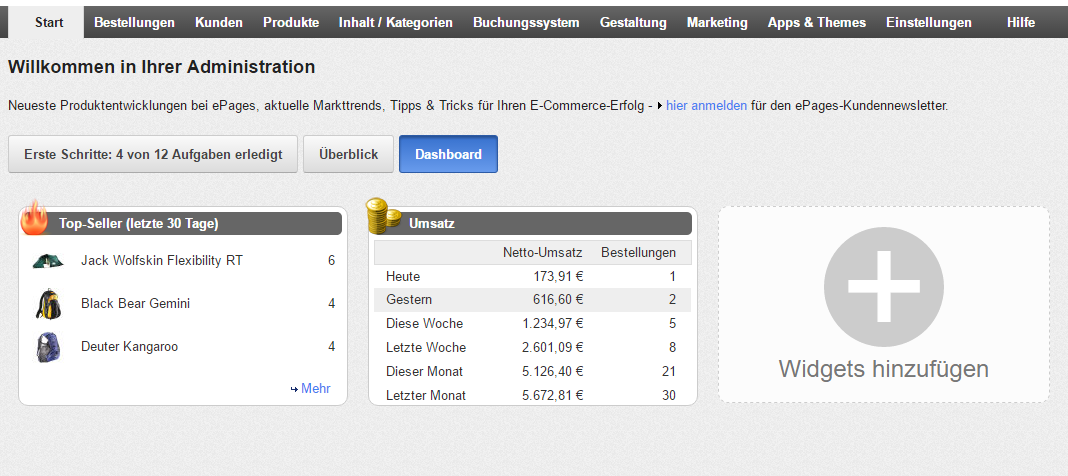
\includegraphics[width=0.9\textwidth]{dashboard.png}
\caption{Widgetauswahl im Dashboard des \acs{MBO}s eines ePages Onlineshops}
\label{fig:dashboard}
\end{center}
\end{figure}
Des Weiteren wurde bereits auf einem zweitägigen firmeninternen Hackathon im Frühjahr 2016 der Versuch der Programmierung einer Statistik-App unternommen, wobei dabei nur mit \gqq{\acs{Mock}-Daten}  hantiert wurde und keine echte Shopanbindung realisiert wurde. Die Ergebnisse zu dieser App sind auf einer internen Wikiseite veröffentlicht und liefern einen ersten Eindruck wie so eine App aussehen könnte und welche Funktionalitäten und Use-Cases ePages vorrangig für solch eine Statistik-App vorsieht. Zu sehen ist ein Menü, über das Bestellungs- und Artikelstatistiken anwählbar sind. In \Abbildung{order} sieht man wie eine graphische Darstellung von Umsätzen pro Bestellung aussehen könnte.

\begin{figure}[htb]
\begin{center}
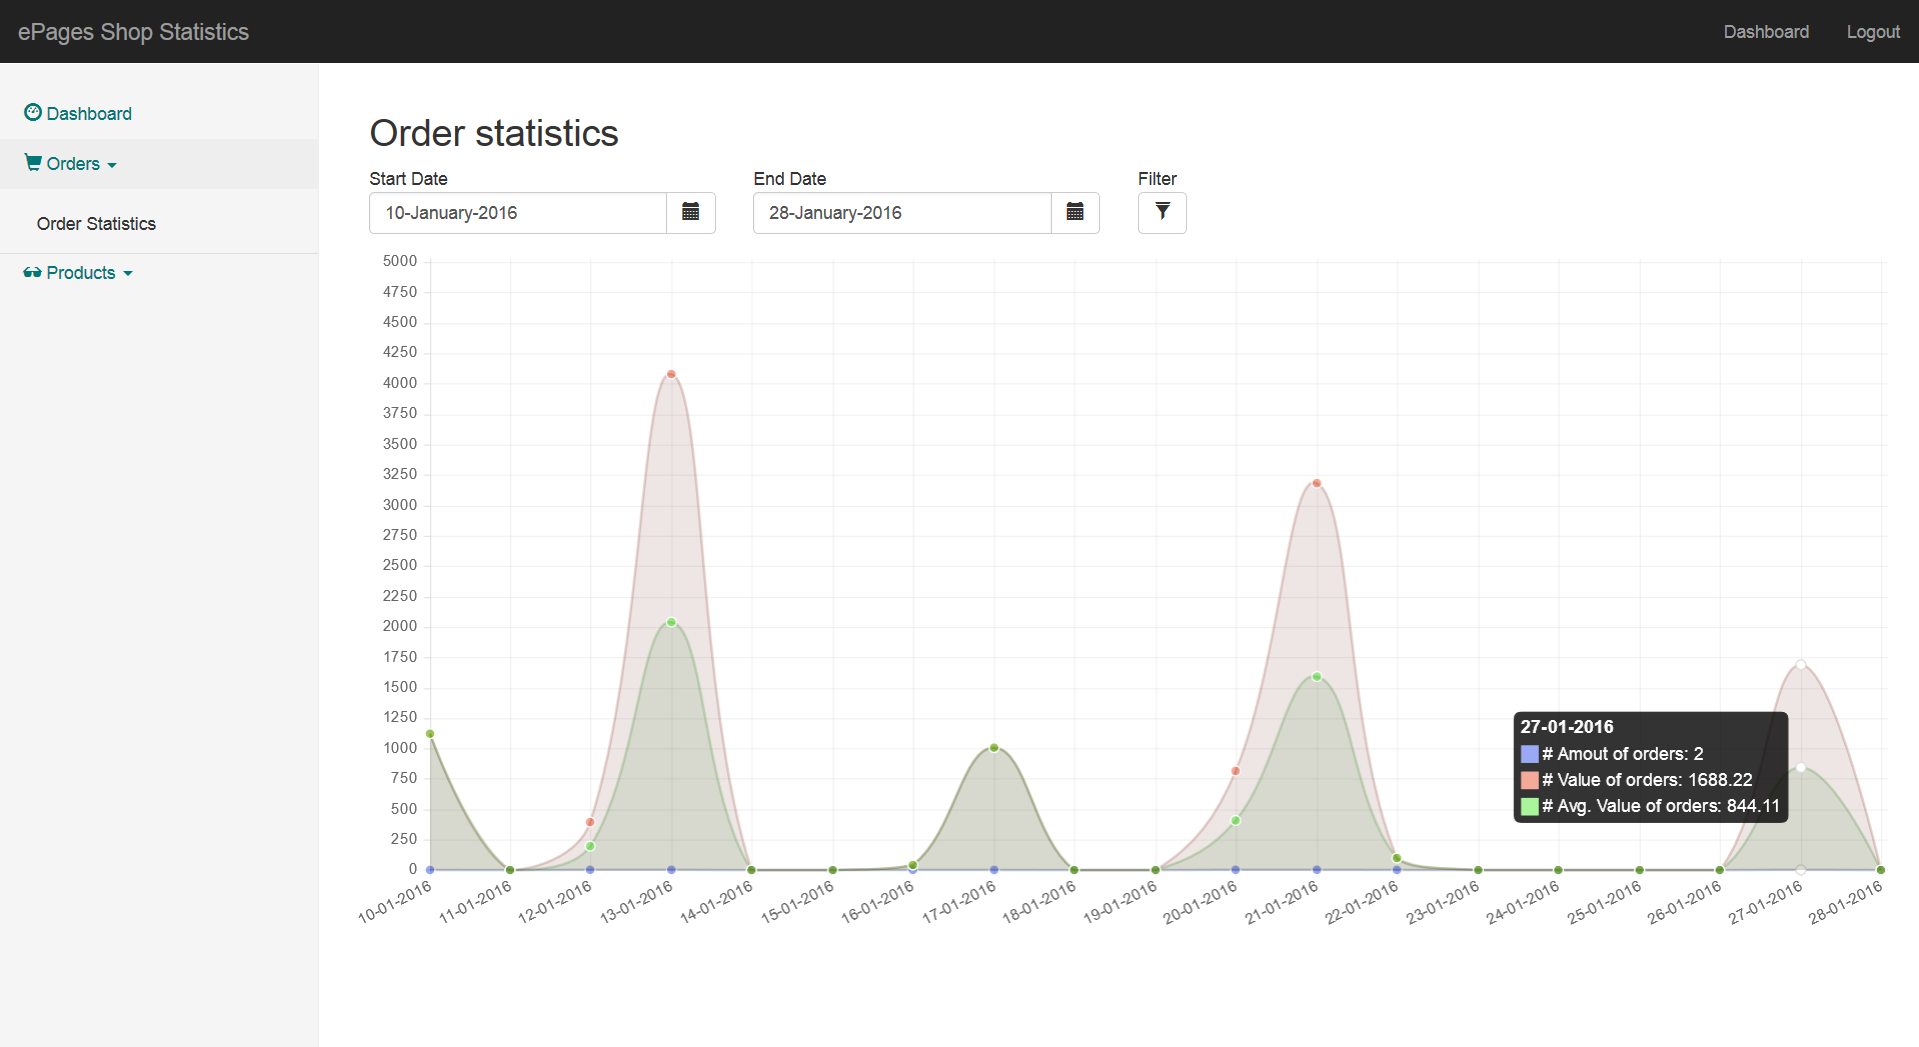
\includegraphics[width=0.7\textwidth, scale=0.5]{epagesapp1.png}
\caption{Graphische Darstellung von Bestellstatistiken}
\label{fig:order}
\end{center}
\end{figure}

\newpage

In \Abbildung{product} werden Artikel mit Gesamtumsatz und Bestellanzahl aufgelistet. Diese Beispiel-App verwendet für das Frontend das AngularJS-Framework \footnote{\url{https://angularjs.org/}} und die Backendskripte sind in Ruby on Rails programmiert. Datenbankanfragen oder angelegte Datenbanken gibt es keine, genauso wenig eine Registrierungs- oder Loginfunktionalität.

\begin{figure}[htb]
\begin{center}
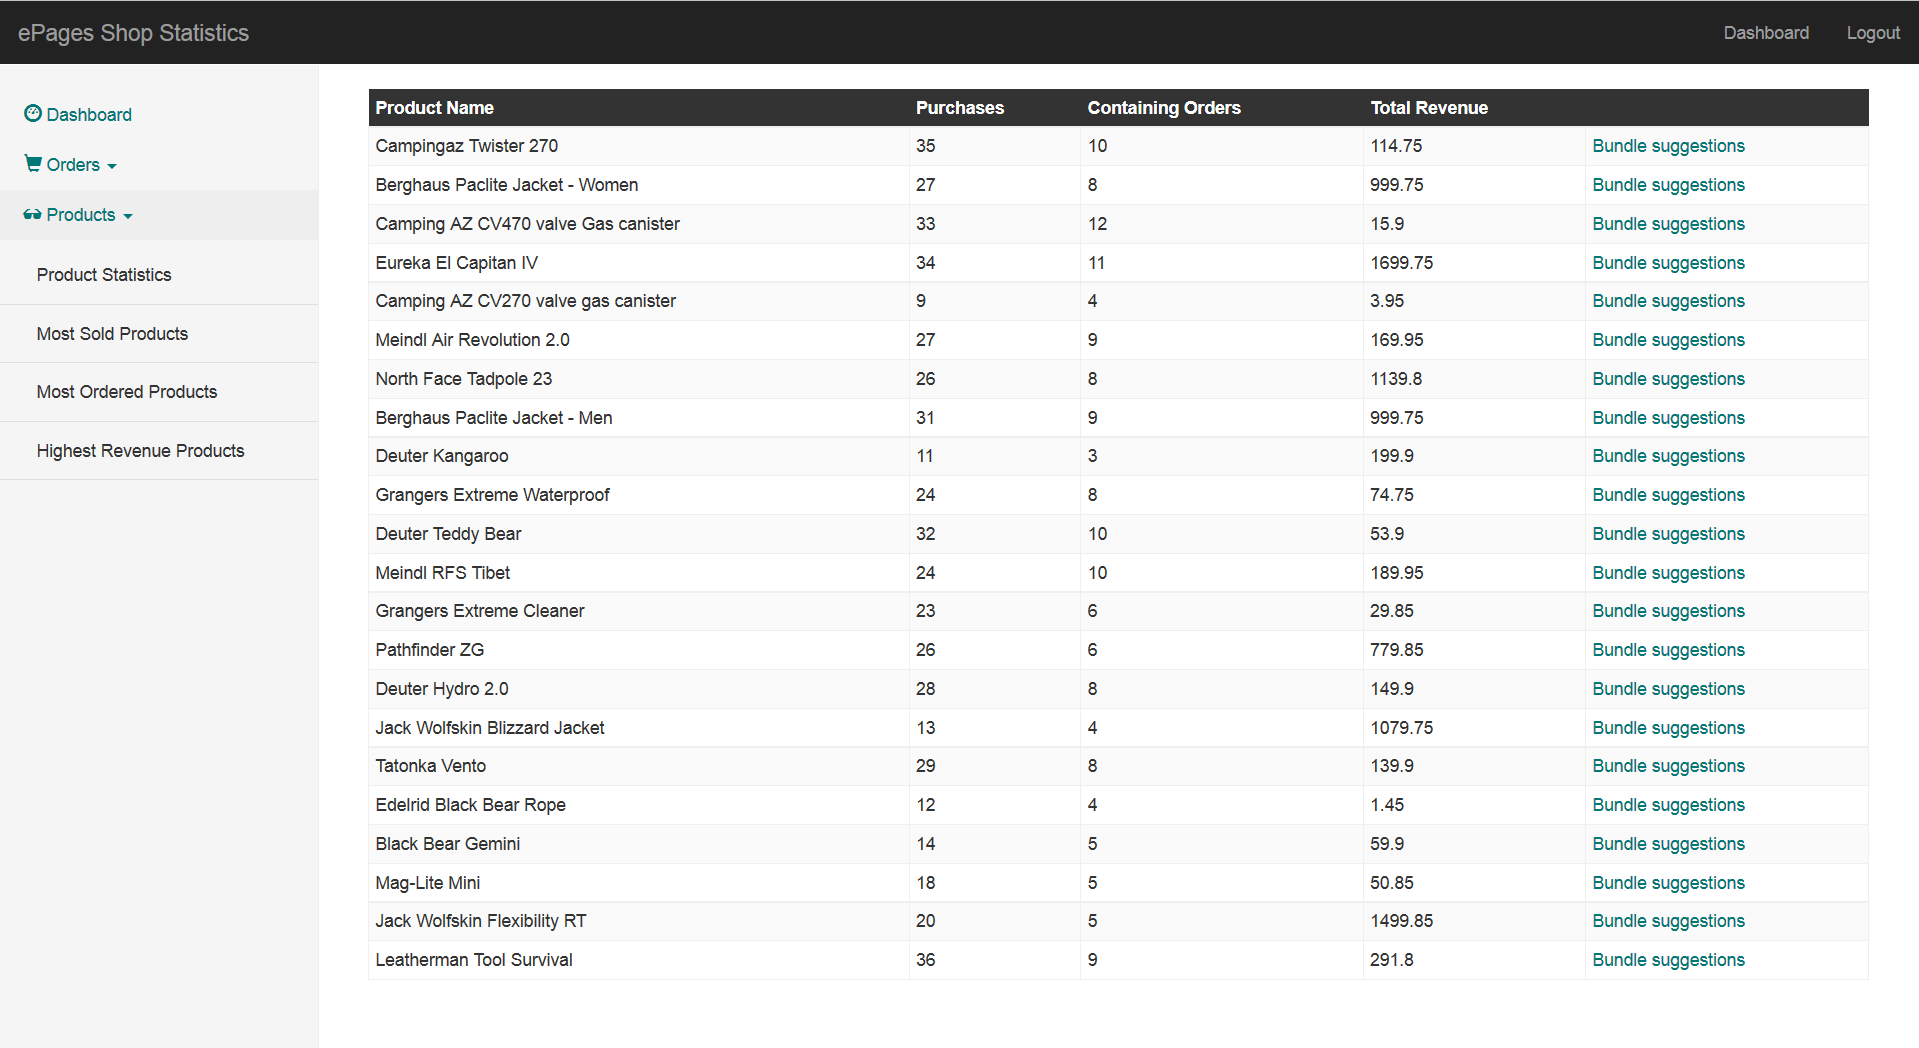
\includegraphics[width=0.7\textwidth, scale=0.5]{epagesapp2.png}
\caption{Auflistung von Artikelstatistiken}
\label{fig:product}
\end{center}
\end{figure}
 
\subsection{Wirtschaftlichkeitsanalyse}
\label{sec:Wirtschaftlichkeitsanalyse}

\subsubsection{\gqq{Make or Buy}-Entscheidung}
\label{sec:MakeOrBuyEntscheidung}

Abgesehen von den im \acs{MBO} hinzufügbaren Statistik-Wigdets
fehlen tiefergehende statistische Analysen und grafische Darstellungen der wichtigsten und interessantesten KPIs, die sich dynamisch über REST-Calls aktualisieren lassen. Darunter fallen die Möglichkeit der Berichterstattung von KPIs pro Kunde und genauere Analysen des Käuferverhaltens (Kaufabbruchrate, Herkunft, Bestellzeiten etc.). Der Wunsch nach einer auf das ePages-System zugeschnittenen App für den ePages-App-Store wurde direkt vom Produktmanagement geäußert und sollte bereits schon mal während eines zweitägigen Hackathons entwickelt werden, was jedoch aufgrund des zu hohem Zeitaufwands für die Entwicklung bei weitem nicht fertig gestellt werden konnte. Durch diese App verspricht sich das Produktmanagement eine höhere Kundenzufriedenheit und damit eine bessere Kundenbindung an die ePages Softwareprodukte sowie längerfristig eine Anwerbung neuer Kunden, die sich durch die Existenz dieser speziellen App vorzugsweise für ePages anstatt für eine andere Onlineshopsoftware entscheiden würden.
\subsubsection{Projektkosten}
\label{sec:Projektkosten}

Die Kosten für die Durchführung des Projektes setzen sich für die 70 Stunden Bearbeitungszeit sowie aus Personal- als auch Ressourcenkosten zusammen.

\paragraph{Berechnung der Entwicklungskosten für ePages}
Laut Arbeitsvertrag liegt meine Ausbildungsvergütung im aktuellen Lehrjahr bei \eur{680} pro Monat. Damit verursache ich der Firma jährliche Kosten in Höhe von 

\begin{equation}
	\eur{680}/\mbox{Monat} \cdot 12 \mbox{Monate/Jahr} = \eur{8160}/\mbox{Jahr}.
\end{equation}

Die Anzahl der Arbeitstage 2016 belaufen sich auf 252 Tage in Thüringen (Jena). Davon stehen mir 25 Urlaubstage zu. Es verbleiben (252 - 25) Tage = 227 Tage vollwertige  achtstündige Arbeitstage. Meine Stundenlohn berechnet sich damit zu

\begin{eqnarray}
	8 \mbox{ h/Tag} \cdot 227 \mbox{ Tage/Jahr} = 1816 \mbox{ h/Jahr} .\\
	\frac{\eur{8160} \mbox{/Jahr}}{1816 \mbox{ h/Jahr}} \approx \eur{4,49}\mbox{/h}.
\end{eqnarray}

Für die Nutzung der Ressourcen\footnote{Laptop, Monitore, Servernutzung, Büro- und Firmenräumlichkeiten, Stromverbrauch, Heizkosten etc.} wird ein pauschaler Stundensatz von \eur{15} angenommen. Für die anderen Mitarbeiter wird pauschal ein Stundenlohn von \eur{25} angenommen. Eine Aufstellung der Kosten befindet sich in Tabelle~\ref{tab:Kostenaufstellung} und sie betragen insgesamt \eur{1844,30}.
\tabelle{Kostenaufstellung}{tab:Kostenaufstellung}{Kostenaufstellung.tex}

\subsubsection{Amortisationsdauer}
\label{sec:Amortisationsdauer}

Geplant ist die fertige App den Nutzern der ePages-Software zur monatlichen Miete zur Verfügung zu stellen. Der Mietpreis wird in dem Bereich $[\mbox{\eur{5}},\mbox{\eur{50}}]$ liegen. Die angenommene Zahl an Nutzern liegt in dem Bereich $[\mbox{1},\mbox{20000}]$.

\paragraph{Berechnung der Amortisationszeit}
Für den Umsatz (=$U$), die diese App abhängig von der Zeit in Monaten (=$t_m$), den Nutzern (=$N$) und von dem Mietpreis pro Monat (=$p_m$) erwirtschaften soll wird die Formel $U = p_m \cdot N \cdot t_m$ zugrunde gelegt. Es wird angenommen, dass die App nach einem Monat 10 Nutzer hat. Dieser Wert wird modellhaft als linear ansteigend mit der Zeit $t_m$ angenommen, d.h. $N = 10 \cdot t_m$. Daraus lässt eine Formel zur Berechnung der Amortisationszeit ($t^{A}_m$) ableiten:

\begin{eqnarray}
	t^{A}_m &=& \frac{U}{p_m \cdot N},\quad \mbox{wobei}\quad U = \mbox{\eur{1844,30},}\quad N = 10 \cdot t_m^{A}\\
	\Rightarrow t^{A}_m &=& \sqrt{\frac{\eur{1844,30}}{10 \cdot p_m}} = 13,58 \cdot p_m^{-\frac{1}{2}}.
\end{eqnarray}

Aus dem Funktionsgraphen aus \Abbildung{AM} lässt sich die Amortisationszeit $t_m^{A}$ für jeden möglichen Mietpreis pro Monat ablesen, wobei die Unsicherheit über das Ergebnis bei kleinen Monatsmietpreisen am geringsten ist, so liegt beispielsweise die Amortisationszeit für \eur{5} Monatsmiete bei ca. 6 Monaten, was durchaus im akzeptablen Budget- bzw. Investitionsrahmen der Firma ist.

\begin{figure}[htb]
\centering
\includegraphicsKeepAspectRatio{graph.png}{0.6}
\caption{Amortisationszeit pro monatlicher Miete}
\label{fig:AM}
\end{figure}

\subsection{Anwendungsfälle}
\label{sec:Anwendungsfaelle}

Die zu entwickelnde App soll die folgenden Anwendungsfälle aus für den Nutzer/Merchant dargestellt in einem Anwendungfalldiagramm \Abbildung{usecase2} mindestens 
realisiert haben.
\begin{figure}[htb]
\centering
\includegraphicsKeepAspectRatio{usecase2.png}{1.0}
\caption{Anwendungsfalldiagramm für die Statistik-App}
\label{fig:usecase2}
\end{figure}


\subsection{Qualitätsanforderungen}
\label{sec:Qualitaetsanforderungen}

Die App soll intuitiv vom Benutzer bedien- bzw. navigierbar sein. Alle dargestellten Statistiken und Berichte sollen selbsterklärend sein. Die App wird als Single-Page-Anwendung programmiert, d.h. bei keiner Aktion des Benutzer soll ein Seitenneuladen ausgelöst werden. Bei Aktualisierung der Daten durch Datenbankabfragen, wenn beispielsweise die Währung oder der Zeitraum geändert wird, sollen alle betroffenen Diagramme und Berichte nahezu gleichzeitig mit den neuen Daten aktualisiert werden. Bei der Datensynchronisation soll der Nutzer eine Rückmeldung darüber erhalten, ob die Synchronisation noch im Gange ist oder nicht oder gar fehlgeschlagen ist.

Zusätzlich soll für jeden Nutzer beim Login eine zeitlich befristete gültige Session gestartet werden, sodass die \acs{URL} für diesen Client einzigartig ist und bei keinem anderen Clientcomputer oder Browser gleichzeitig verwendet werden kann. Das Design sollte für den Nutzer ansprechend sein und die App sollte in Ansätzen \gqq{responsive} sein, um auch auf mobilen Geräten benutzbar sein zu können.
Die App soll frontend- und backendseitig modular aufgebaut sein, so dass Fehlerbeseitigung oder Modifizierungen schnell und übersichtlich möglich sind und sich konsistent in das Gesamtprogramm einfügen.
Der Programmcode sollte strukturiert nach gängigen oder firminternen Code-Conventions sein und an allen wichtigen Stellen Kommentare für Entwickler enthalten.


\subsection{Lastenheft/Fachkonzept}
\label{sec:Lastenheft}

Die Anwendung muss folgende Anforderungen erfüllen:
\begin{enumerate}
\item Registrierungsmechanismus
\begin{enumerate}
\item Der Nutzer muss Vorname, Name, Email-Adresse, Passwort und seine Shop-\acs{URL} zur Registrierung eingeben können.
\item Die Passworteingabe sollte blicksicher sein und verifiziert werden.
\item Nach der Registrierung bekommt man eine Erfolgsmeldung und wird auf die Loginseite weitergeleitet.
\end{enumerate}
\item Login-Mechanismus
\begin{enumerate}
\item Die Logindaten sollen die Email-Adresse und das Passwort sein.
\item Bei Falscheingabe von Email-Adresse oder Passwort soll eine entsprechende Rückmeldung erfolgen.
\end{enumerate}
\item Logout-Mechanismus
\begin{enumerate}
\item Im Nutzerbereich der App soll eine Möglichkeit zum Beenden der Session/Logout geschaffen werden.
\item Beim Ausloggen soll die Session beendet und eine Weiterleitung auf den Loginbereich erfolgen.
\end{enumerate}
\item Navigation im Nutzerbereich
\begin{enumerate}
\item Alle wesentlichen Benutzerinteraktionen der App sollen nur über ein einziges Navigationspanel entweder an der Seite oder oben als Leiste durchführbar sein.
\item Die Navigation sollte einen logischen und intuitiven Aufbau haben und sollte vom Design her einheitlich sein.
\end{enumerate}
\item Graphische Darstellungen statistischer Auswertungen
\begin{enumerate}
\item Die Umsätze und Bestellungen im Onlineshop sollen wahlweise als Balken- oder Liniendiagramme darstellbar sein.
\item Für die Diagramme soll der Zeitraum auswählbar über die Menüleiste sein. Die auswählbaren Zeiträume sollen mindestens die einzelnen Kalenderwochen, Monate und Jahre umfassen.
\item Es soll möglich sein, die Diagramme wahlweise aufgrund von Brutto - oder Nettoumsätzen anzuzeigen.
\end{enumerate}
\item Währungsfilter
\begin{enumerate}
\item Die Anzeige der Statistiken und Berichte sollte abhängig von der  ausgewählten Währung sein, da im Onlineshop mehrere Währungen eingestellt sein können.
\item Hierzu muss eine Auswahlmöglichkeit über einen Währungsfilter geschaffen werden.
\end{enumerate}
\item Datensynchronisation
\begin{enumerate}
\item Es soll die Möglichkeit für den Nutzer geschaffen werden über einen \gqq{Button} die Datensynchronisation zwischen seinem Shop und der App auszulösen, falls der Nutzer eine neuerliche Synchronisation für notwendig hält.
\item Der Nutzer soll eine Rückmeldung über den Prozess der Synchronisation bekommen und eine entsprechende Mitteilung falls die Synchronisation fehlgeschlagen ist.
\item Die Daten sollen über \acs{REST}-Calls unter Verwendung der ePages \acs{REST-API} vom Onlineshop angefordert und in einer \acs{MySQL}-Datenbank abgespeichert werden.
\end{enumerate}
\item Datenbank
\begin{enumerate}
\item Zum Aktualisieren der App-Statistiken durch Benutzerinteraktionen abseits der Datensynchronisation sollen keine \acs{REST}-Calls mehr ausgelöst werden, um die ePages-REST-API nicht zu sehr zu belasten. Vielmehr sollen hier die benötigten Daten aus der Datenbank abgefragt werden.
\item Es soll ein Datenbankmodell in der 3. Normalform entworfen werden.
\end{enumerate}
\item Umsatzstatistik nach Bundesland
\begin{enumerate}
\item Es soll über ein Tortendiagramm möglich sein, die Umsatzverteilung pro Bundesland angezeigt zu bekommen.
\item Außerdem sollen Shopkunden dabei berücksichtigt werden, denen kein Bundesland zugewiesen ist oder die im Ausland wohnen.
\end{enumerate}
\item Darstellung umsatzstärkster Kunden
\begin{enumerate}
\item Die App soll in tabellarischen Stil die Kunden geordnet nach Umsatz auflisten mit Namen, Email-Adresse, Gesamtumsatz, Gesamtzahl an Bestellungen und letztem Bestelldatum.
\item Die Erstellung der Tabelle sollte dynamisch erfolgen.
\end{enumerate}
\item Design
\begin{enumerate}
\item Die gesamte App sollte zumindest ein grundlegendes responsives Verhalten aufgrund des 12er-Grid-Systems zeigen.
\end{enumerate}
\end{enumerate}




% !TEX root = ../Projektdokumentation.tex
\section{Entwurfsphase} 
\label{sec:Entwurfsphase}

\subsection{Zielplattform}
\label{sec:Zielplattform}

Die Statistik-App wird als Web-Applikation entwickelt und sollte damit lauffähig in allen gängigen Internetbrowsern eines jeden Heim-PCs oder Laptops sein, mindestens jedoch im Internet-Explorer, Firefox und Google-Chrome. Die App ist über eine feste acs{URL} auf dem \textit{uberspace.de}-Server erreichbar. Die Wahl auf \textit{uberspace} als Host fiel aufgrund der geringen monatlichen Mietkosten für das Hosting und die Servernutzung und der Unterstützung von \acs{MySQL}. Die verwendeten Programmiersprachen umfassen Javascript und \acs{PHP}. Dies ist der Tatsache geschuldet, dass viele meiner Kollegen und mein Ausbilder ein großes Know-how in diesen Sprachen haben und mich so effektiv unterstützen können. Des Weiteren ist für mich als Auszubildender in der Frontendentwicklung Javascript die Programmiersprache, in der ich mich am besten auskenne.

Die Wahl auf \acs{PHP} als serverseitige Sprache fiel aufgrund der großen Community im Vergleich zu \acs{NodeJS} und der einfachen Datenbankanbindung an eine MySQL-Datenbank, siehe hierzu \cite{PHP}. NodeJS wird zwar für Single-Page-Anwendungen empfohlen, jedoch sollte man für rechenintensive Anwendungen, wie die Statistik-App eine ist, dann doch eher auf PHP zurückgreifen. Zudem gibt es von ePages auf der App-Entwicklungs-Webseite Tutorials zur App-Entwicklung in PHP und auch bereits eine eigene PHP-Klasse zur Anforderung von \acs{REST}-Daten. Prinzipiell hätte man für diese Anwendung auch \acs{MongoDB} als Datenbanksystem nehmen können. Das Vorhaben wurde aber mangels Erfahrung im Umgang damit verworfen.

\subsection{Architekturdesign}
\label{sec:Architekturdesign}

Die Frontendarchitektur der App wird unter Verwendung des Javascript-Frameworks ReactJS realisiert. ReactJS hat Ähnlichkeiten zu traditionellen \acs{MVC}-Frameworks, fokussiert sich jedoch besonders auf die Idee eine Website aus einzelnen interaktiven Komponenten zusammengebaut zu betrachten, die voneinander abhängig sein können (über Eltern-Kind-Beziehungen) und immer einen definierten (Daten-) Zustand haben, der sich dynamisch in Echtzeit ohne erneutes Laden der gesamten Website ändern kann.
Die Statistik-App soll genau diesen Ansprüchen entsprechen, da die einzelnen Diagramme, Tabellen und Interaktionsmöglichkeiten jeweils als eigenständige Komponenten bzw. Module aufgefasst werden können, die alle einen vordefinierten Zustand haben, der sich durch Interaktionen des Nutzers ändern kann.

Dadurch fiel die Wahl schnell auf ReactJS als modernes Framework mit groß gewachsener Community und dessen Fokus auf zustandsbehaftete Anwendungen. Zudem wird es bereits innerhalb ePages für das neue Softwareprodukt verwendet, sodass auch hier schon ein hilfreiches Know-how vorhanden ist. Nicht zuletzt erleichtert ReactJS die modularisierte Programmierung mit Javascript, durch Einführung von Komponenten die alle von einer Basiskomponente abgeleitet sind. Außerdem unterstützt ReactJS die Verwendung von ECMAScript 6, wodurch nun auch mit Javascript eine emulierte objektorientierte Programmierung möglich ist.

Für die graphischen Darstellungen wird die Javascript-Bibliothek C3.js verwendet, welche kostenlos ist und von der extrem mächtigen D3.js-Bibliothek abgeleitet ist. C3.js bietet gerade den nötigen Umfang an Einstellungen, Darstellungsmöglichkeiten und Beispielen für die Statistik-App. Es gibt zwar wesentlich bessere und umfangreichere Bibliotheken für graphische Darstellungen, die meisten davon sind jedoch mindestens ab der kommerziellen Nutzung der App kostenpflichtig.

Serverseitig fiel die Entscheidung auf das \acs{PHP}-Slim-Framework auf Anraten von Kollegen. Slim ist extra für Webanwendungen entwickelt worden, die mit vielen \acs{REST}-Requests hantieren müssen und bietet einen schnellen und einfachen Einstieg in diese Grundfunktionalitäten, auf die es hier serverseitig für die App ankommt.

Die Kommunikation zwischen Frontend- und Backendskripten findet mittels \acs{AJAX} statt, wodurch bei Serveranfragen ein Neuladen oder Ausbremsen der Interaktionen mit der Seite verhindert werden.

Um die App ansatzweise \gqq{responsive} zu gestalten, wird das \acs{CSS}-Framework Materialize \footnote{\url{http://materializecss.com/}} verwendet. Es bietet darüber hinaus vorgefertigte Designs und Javascript-Interaktionen für Navigationsleisten, Menüs, Buttons etc., welche in der App dann auch verwendet werden.

\subsection{Datenmodell}
\label{sec:Datenmodell}
Das verwendete Datenmodell ist in \Abbildung{erm2} als \acs{ERM} dargestellt. Dort sind insbesondere die Beziehungen und Kardinalitäten zwischen den Entitäten Shop, Kunde, Bestellung, Artikel, Kundenadresse usw. dargestellt.  
\begin{figure}[htb]
\centering
\includegraphicsKeepAspectRatio{erm2.png}{1.0}
\caption{ER-Modell: Beziehungen und Kardinalitäten zwischen den Entitäten}
\label{fig:erm2}
\end{figure}
\subsection{Geschäftslogik}
\label{sec:Geschaeftslogik}

Der Kern der Geschäftslogik liegt in den Programmabläufen der Frontendskripte, die abhängig von den Benutzerinteraktionen mit der App beim Client in den einzelnen React-Komponenten ablaufen und gegebenfalls \acs{AJAX}-POST-Request zur (Daten-) Zustandsaktualisierung an den Server senden, bei dem Skripte für entsprechende Datenbankabfragen ablaufen. Exemplarisch sei hier die geplante Logik des Synchronisationsprozesses zwischen dem Onlineshop und der App anhand eines Sequenzdiagramms in \Anhang{app:sequenz} dargelegt.

Der Prozess soll durch ein Klickereignis auf den SYNC-Button in der Menüleiste ausgelöst werden, infolgedessen wird ein AJAX-Request an den Server gestellt, der sich wiederum per REST-calls die aktuellen Shopdaten holt und in die Datenbank einträgt.

Alle weiteren Klickereignisse, die der Nutzer über das Menü auslösen kann, sollen dann wenn notwendig nur noch Datenbankabfragen auslösen und keine weiteren REST-calls, um die REST-Schnittstelle zu schonen und die Abfrage- und Verarbeitungsprozesse zu beschleunigen.

\paragraph{Logik der Frontendarchitektur}
Die Statistik-App wird als Single-Page-Anwendung entwickelt, d.h. an keiner Stelle der App wird ein Neuladen der Seite ausgelöst. Dies wird durch React-Komponenten realisiert, die über Eltern-Kind-Beziehungen miteinander verknüpft sind. Dabei besitzt jede Komponente einen (Daten-)Zustand, der konstant oder veränderlich sein kann je nachdem, ob Daten aktualisiert werden oder nicht. Die Aktualisierung des Datenzustands findet ausschließlich asynchron statt, um während dieses Vorgangs die Benutzbarkeit der App nicht einzuschränken. Zusätzlich zum Zustand können jeder Kindkomponente von der Elternkomponente sogenannte \gqq{props} (properties/Eigenschaften) übergeben werden ähnlich zu dem Vererbungsprozess in der objektorientierten Programmierung bei abgeleiteten Klassen mit dem Unterschied, dass die Kindkomponente nicht automatisch alle Zustandsattribute und Methoden der Elternkomponent erbt, sondern nur jene, die ihr direkt zur Verwendung zugewiesen bzw. weitergereicht wurden, d.h. die übergebenen props können sowohl Zustandsattribute wie auch Methoden der Elternkomponente sein.

Der architektonische Frontendaufbau über die React-Komponenten und deren Abhängigkeiten zueinander ist in \Anhang{app:classes} dargestellt. 

Ähnlich zu einem \acs{UML}-Klassendiagramm zeigen die Pfeile in Richtung der Elternkomponente, von der \gqq{geerbt} wird. Die Basiskomponente, von der alle anderen Komponenten aufgerufen werden, ist die \textbf{RoutedContent}-Komponente, in der über die React-Router-Komponente/Bibliothek die URL-Routen zu den anderen Basiskomponenten definiert werden. Jede Komponente in der Abbildung besitzt einen Eintrag \textbf{state attributes}, der alle Zustandsdaten, falls vorhanden, auflistet. Diese Daten definieren den Zustand der Komponente. Zusätzlich werden alle in den Komponenten implementierten Methoden aufgelistet, die als props auch an Kindkomponenten weitergereicht werden können. Falls eine Komponente auch props übergeben bekommt, so werden jene übergebenen props zusätzlich auch noch aufgelistet.

\subsection{Maßnahmen zur Qualitätssicherung}
\label{sec:Qualitaetssicherung}

Um die Umsetzung aller Qualitätsanforderungen aus \ref{sec:Qualitaetsanforderungen} abzusichern, werden ständig händische Entwicklertests in verschiedenen Browsern durchgeführt, die darauf ausgerichtet sind, die Gesamtfunktionalität der App bei jeder neuen Implementierung oder Code-Änderung nicht zu gefährden. Zuletzt wird die teaminterne \acs{QA}-Abteilung damit beauftragt alle genannten Qualitätsanforderungen durchzutesten. Automatische Tests sind für dieses Projekt nicht vorgesehen.

% !TEX root = ../Projektdokumentation.tex
\section{Implementierungsphase} 
\label{sec:Implementierungsphase}

\subsection{Verwendete Bibliotheken und Tools}
\label{sec:Tools}
Der Einstiegspunkt für die gesamte App ist die \textit{index.php}-Datei zu sehen im \Anhang{app:index}. Die verwendeten Javascript-Dateien für die App umfassen die JQuery-Bibliothek, die darauf aufbauende Materialize-Bibliothek als CSS-Framework und die Haupt-Javascript-Datei \textit{main.js}, welche im \textit{build}-Ordner liegt. Diese Datei enthält die gesamte ReactJS-Logik und die gebauten Komponenten. Erzeugt wurde sie durch einen Gulp-Task. Gulp \footnote{http://gulpjs.com} ist ein Task Runner, der häufig in Verbindung mit ReactJS eingesetzt wird. Alle benötigten Bibliotheken liegen lokal vor und sind damit unabhängig von einer vorhandenen Netzwerkverbindung.

\subsection{Implementierung der Datenstrukturen}
\label{sec:ImplementierungDatenstrukturen}

Ausgangspunkt hierfür ist das Datenmodell aus \ref{sec:Datenmodell}, welches Anlass zur Erstellung der in \Anhang{app:datenbank} aufgeführten miteinander in Verbindung stehenden Tabellen hat. Primär- und Fremdschlüssel sind entsprechend gekennzeichnet. Man beachte, dass zwischen dem Onlineshop und dem Kunden eine m:n Beziehung besteht, da ein Kunde in verschiedenen Onlineshops einkaufen kann, sodass hier eine Zwischentabelle vonnöten ist. Die Tabelle für die Artikel/Produkte wird nur pro forma angelegt, da diese während der Dauer des Projekts noch nicht mit Daten gefüllt werden kann, sodass auch keine Beziehungen zu den anderen Tabellen hergestellt werden können. Die Tabelle tbl\_states gibt Auskunft darüber, ob und in welchem Bundesland der Kunde wohnhaft ist. Die Anbindung an den Shop geschieht über das Attribut shop\_url und dem besonders geheimzuhaltenden access\_token aus der Tabelle tbl\_shop, der während des Registrierungsprozesses von epages erzeugt und automatisch in der App-Datenbank abgelegt wird.

Die Erstellung der Tabellen wird unter Verwendung des Datenbank-Management-Systems \textit{phpMyAdmin} \footnote{https://www.phpmyadmin.net/} durchgeführt, was sehr einfach und intuitiv zu bedienen ist und daher auch für die Verwaltung der Tabellen und deren Daten verwendet wird. Eine Screenshot von den in \textit{phpMyAdmin} angelegten Tabellen ist im \Anhang{app:phpmyadmin} zu sehen.

\subsection{Implementierung der Benutzeroberfläche}
\label{sec:ImplementierungBenutzeroberflaeche}

\paragraph{Loginbereich} Für die Benutzeroberfläche des Login- und Registrierungsbereichs wird sich an diverser anderer Apps orientiert. Dabei fiel auch die Wahl auf die zu verwendende Schriftart \gqq{Dosis:700}, die in vielen modernen Apps zur Anwendung kommt.
\begin{figure}[htb]
\centering
\includegraphicsKeepAspectRatio{login.png}{0.7}
\caption{Design und Aufbau des Loginbereichs}
\label{fig:loginbereich}
\end{figure} 
Wie in \Abbildung{loginbereich} zu erkennen sind alle Texte in Deutsch verfasst. Dies wird innerhalb dieses Projekt für die gesamte App gelten. Über eine Lokalisierung und Unterstützung mehrerer Sprachen kann man sich abseits dieses Projektes später Gedanken machen.
\newpage
\paragraph{Header im Nutzerbereich}
Die Implementierung des Headers im Nutzerbereich nach erfolgreichem Einloggen in die App ist in \Abbildung{nutzerbereich} zu sehen.
\begin{figure}[htb]
\centering
\includegraphicsKeepAspectRatio{navigation.png}{1.0}
\caption{Design und Aufbau des Headers im Benutzerbereich}
\label{fig:nutzerbereich}
\end{figure}
Alle Interaktionen des Benutzers mit der App sollen über die Menüleiste über davon zugängliche Dropdown-Felder oder Buttons erfolgen wie in \Abbildung{dropdown} zu erkennen. Mittig oben erscheint der Shopname des Nutzers, links oben eine Willkommensnachricht und rechts oben die Möglichkeit zum Ausloggen.
 \begin{figure}[htb]
\centering
\includegraphicsKeepAspectRatio{dropdown.png}{1.0}
\caption{Beispiel eines Dropdown-Feldes nach einem Klickereignis}
\label{fig:dropdown}
\end{figure}
\paragraph{Anzeige der Statistiken}
Im Nutzerbereich werden dem Shopbesitzer insgesamt drei Diagramme angezeigt, zwei sind in \Abbildung{umsatz} zu sehen.
\begin{figure}[htb]
\centering
\includegraphicsKeepAspectRatio{sales.png}{1.0}
\caption{Diagramme für statistische Auswertungen}
\label{fig:umsatz}
\end{figure}
Die Balkendiagramme stellen den Umsatz für die ausgewählte Währung pro Tag, Woche, Monat oder Jahr dar je nach Auswahl des Nutzers. Das Tortendiagramm schlüsselt den Gesamtumsatz nach Bundesländer auf, wobei alle ausländischen oder nicht zugeordneten Umsätze unter die Kategorie \gqq{Andere} fallen. Ein drittes hier nicht sichtbares Diagramm stellt die Anzahl der Bestellungen pro gewähltem Zeitraum dar und zeigt zusätzlich an, ob diese schon bezahlt sind oder nicht.

Des Weiteren wird weiter unten eine Tabelle angezeigt, die die zehn umsatzstärksten Kunden sortiert nach Umsatz auflistet.
\begin{figure}[htb]
\centering
\includegraphicsKeepAspectRatio{tttable.png}{1.0}
\caption{Top-Ten-Tabelle der umsatzstärksten Kunden}
\label{fig:umsatz}
\end{figure}

\subsection{Implementierung der Geschäftslogik}
\label{sec:ImplementierungGeschaeftslogik}

Exemplarisch wird hier die Implementierung des Synchronisationsprozesses aus \Anhang{app:sequenz} aufgeführt. Der Code dazu ist im Anhang zu finden. Nach einem Klick auf den SYNC-Button wird zunächst die Funktion \textit{loadSalesData()} aufgerufen, siehe \Anhang{app:loadsales}. Diese löst einen AJAX-Request an den Server aus. Dort wird die Funktion \textit{handleLoadShopData()} aufgerufen, siehe \Anhang{app:loadsalesphp}, welche REST-calls zum Shop des App-Nutzers abgesetzt, um alle relevanten Shop- und Bestelldaten zu holen, die dann in die Datenbank eingefügt werden.
Anschließend wird bei erfolgreicher Ausführung des AJAX-Requests in der \textit{done()}-Methode die Funktion \textit{loadCurrentSales(event, month, year, tax, paidOrders, currency, currencySymbol)} aufgerufen, welche sich über mehrere AJAX-Requests alle aktuellen Daten für die Appstatistiken aus der Datenbank beschafft und diese an die Komponenten zur Aktualisierung ihrer Datenzustände und zwecks Neuladens weiterreicht.  

\subsection{Implementierung des Session-Managements}
\label{sec:Session}

Bei erfolgreichem Einloggen des Nutzers wird eine Weiterleitungs-URL aus einem Cookie und einem Serversessiontoken zusammengebaut, wie in \Abbildung{cookie} zu sehen. Der Cookie ist acht Stunden lang gültig. Auf der App-Komponente angelangt, wird der Sessiontoken auf dem Server nochmal gegengeprüft. Erst nach erfolgreicher Prüfung wird die App-Komponente geladen. 
\begin{figure}[htb]
\centering
\includegraphicsKeepAspectRatio{cookie.png}{1.0}
\caption{Cookiesetzung in der Login-Komponente}
\label{fig:cookie}
\end{figure}
Beim Ausloggen wird der Sessiontoken auf dem Server gelöscht und der Nutzer wird auf die Login-Komponente umgeleitet. Damit wird die Session-URL ungültig gemacht.
% !TEX root = ../Projektdokumentation.tex
\section{Abnahmephase} 
\label{sec:Abnahmephase}

\begin{itemize}
	\item Welche Tests (\zB Unit-, Integrations-, Systemtests) wurden durchgeführt und welche Ergebnisse haben sie geliefert (\zB Logs von Unit Tests, Testprotokolle der Anwender)?
	\item Wurde die Anwendung offiziell abgenommen?
\end{itemize}

\paragraph{Beispiel}
Ein Auszug eines Unit Tests befindet sich im \Anhang{app:Test}. Dort ist auch der Aufruf des Tests auf der Konsole des Webservers zu sehen.


\Zwischenstand{Abnahmephase}{Abnahme}

% !TEX root = ../Projektdokumentation.tex
\section{Dokumentation}
\label{sec:Dokumentation}

\begin{itemize}
	\item Wie wurde die Anwendung für die Benutzer/Administratoren/Entwickler dokumentiert (\zB Benutzerhandbuch, \acs{API}-Dokumentation)?
	\item Hinweis: Je nach Zielgruppe gelten bestimmte Anforderungen für die Dokumentation (\zB keine IT-Fachbegriffe in einer Anwenderdokumentation verwenden, aber auf jeden Fall in einer Dokumentation für den IT-Bereich).
\end{itemize}

\paragraph{Beispiel}
Ein Ausschnitt aus der erstellten Benutzerdokumentation befindet sich im \Anhang{app:BenutzerDoku}.
Die Entwicklerdokumentation wurde mittels PHPDoc\footnote{Vgl. \cite{phpDoc}} automatisch generiert. Ein beispielhafter Auszug aus der Dokumentation einer Klasse findet sich im \Anhang{app:Doc}. 

\Zwischenstand{Dokumentation}{Dokumentation}

% !TEX root = ../Projektdokumentation.tex
\section{Fazit} 
\label{sec:Fazit}

\subsection{Soll-/Ist-Vergleich}
\label{sec:SollIstVergleich}

\begin{itemize}
	\item Wurde das Projektziel erreicht und wenn nein, warum nicht?
	\item Ist der Auftraggeber mit dem Projektergebnis zufrieden und wenn nein, warum nicht?
	\item Wurde die Projektplanung (Zeit, Kosten, Personal, Sachmittel) eingehalten oder haben sich Abweichungen ergeben und wenn ja, warum?
	\item Hinweis: Die Projektplanung muss nicht strikt eingehalten werden. Vielmehr sind Abweichungen sogar als normal anzusehen. Sie müssen nur vernünftig begründet werden (\zB durch Änderungen an den Anforderungen, unter-/überschätzter Aufwand).
\end{itemize}

\paragraph{Beispiel (verkürzt)}
Wie in Tabelle~\ref{tab:Vergleich} zu erkennen ist, konnte die Zeitplanung bis auf wenige Ausnahmen eingehalten werden.
\tabelle{Soll-/Ist-Vergleich}{tab:Vergleich}{Zeitnachher.tex}


\subsection{Lessons Learned}
\label{sec:LessonsLearned}

\begin{itemize}
	\item Was hat der Prüfling bei der Durchführung des Projekts gelernt (\zB Zeitplanung, Vorteile der eingesetzten Frameworks, Änderungen der Anforderungen)?
\end{itemize}


\subsection{Ausblick}
\label{sec:Ausblick}

\begin{itemize}
	\item Wie wird sich das Projekt in Zukunft weiterentwickeln (\zB geplante Erweiterungen)?
\end{itemize}


% Literatur ------------------------------------------------------------------
\clearpage
\renewcommand{\refname}{Literaturverzeichnis}
\bibliography{Bibliographie}
\bibliographystyle{Allgemein/natdin} % DIN-Stil des Literaturverzeichnisses

% Anhang ---------------------------------------------------------------------
\clearpage
\appendix
\pagenumbering{roman}
% !TEX root = Projektdokumentation.tex
\section{Anhang}
\subsection{Detaillierte Zeitplanung}
\label{app:Zeitplanung}

\tabelleAnhang{ZeitplanungKomplett}

\subsection{Vergleich zwischen geplanter und tatsächlich gebrauchter Zeit}
\label{app:ZeitplanungReal}

\tabelleAnhang{ZeitplanungKomplettReal}
\clearpage

\subsection{Ausschnitt aus der Tabellenstruktur in phpMyAdmin}
\label{app:phpmyadmin}
\begin{center}
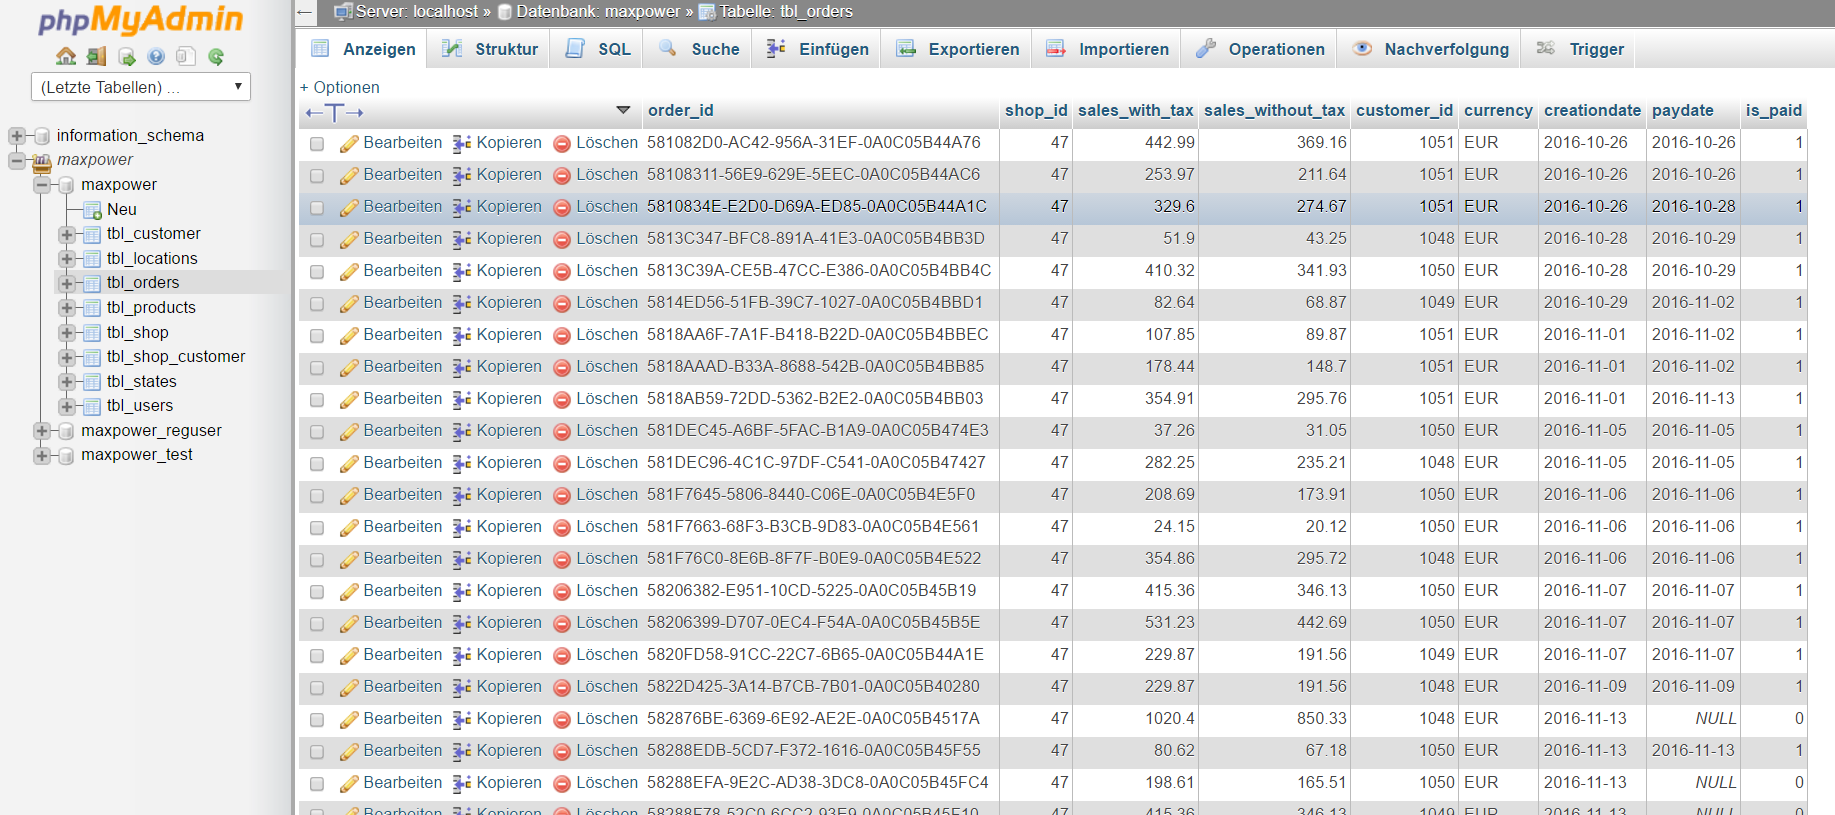
\includegraphics[page=1, width=1.0\textwidth]{myadmin.png}
\end{center}
\subsection{Datenbankmodell für die MySQL-Datenbanktabellen}
\label{app:datenbank}
\begin{center}
\includegraphics[page=1, width=1.0\textwidth]{data.png}
\end{center}
\subsection{Sequenzdiagramm zum Synchronisationsprozess}
\label{app:sequenz}
\begin{center}
\includegraphics[page=1, width=1.0\textwidth]{seq2.png}
\end{center}
\subsection{React-Komponenten-Architektur und Abhängigkeiten}
\label{app:classes}
\begin{center}
\includegraphics[page=1, width=1.1\textwidth]{classes2.png}
\end{center}
\subsection{Einstiegspunkt für die Single-Page-App}
\label{app:index}
\begin{center}
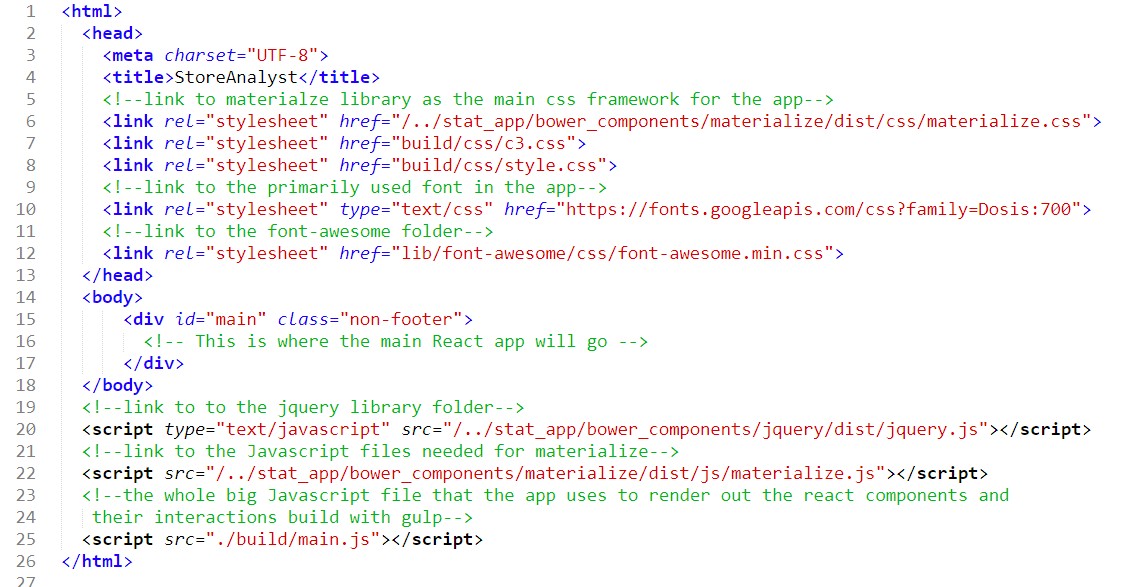
\includegraphics[page=1, width=1.0\textwidth]{index.png}
\end{center}
\subsection{Clientseitige Abhandlung der Synchronisation}
\label{app:loadsales}
\begin{center}
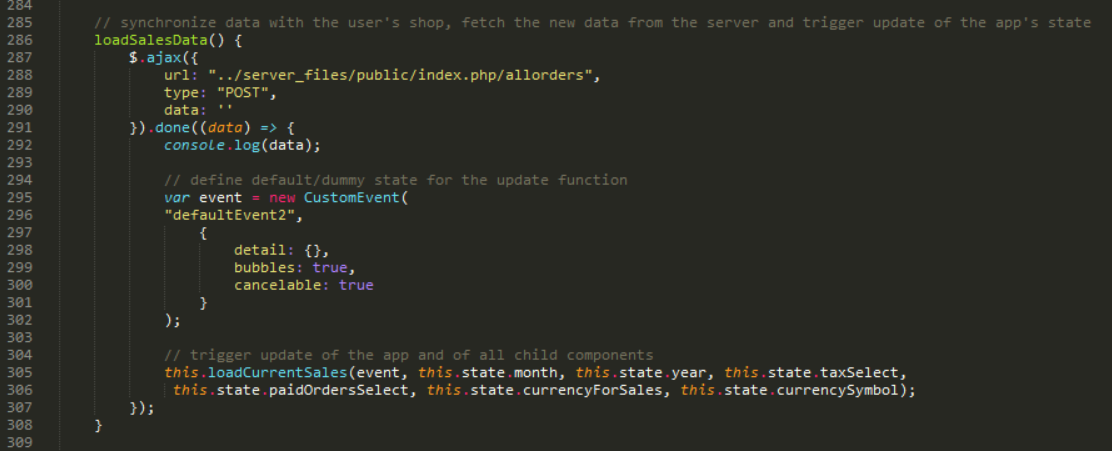
\includegraphics[page=1, width=1.0\textwidth]{loadsales.png}
\end{center}
\subsection{Serverseitige Abhandlung der Synchronisation}
\label{app:loadsalesphp}
\begin{center}
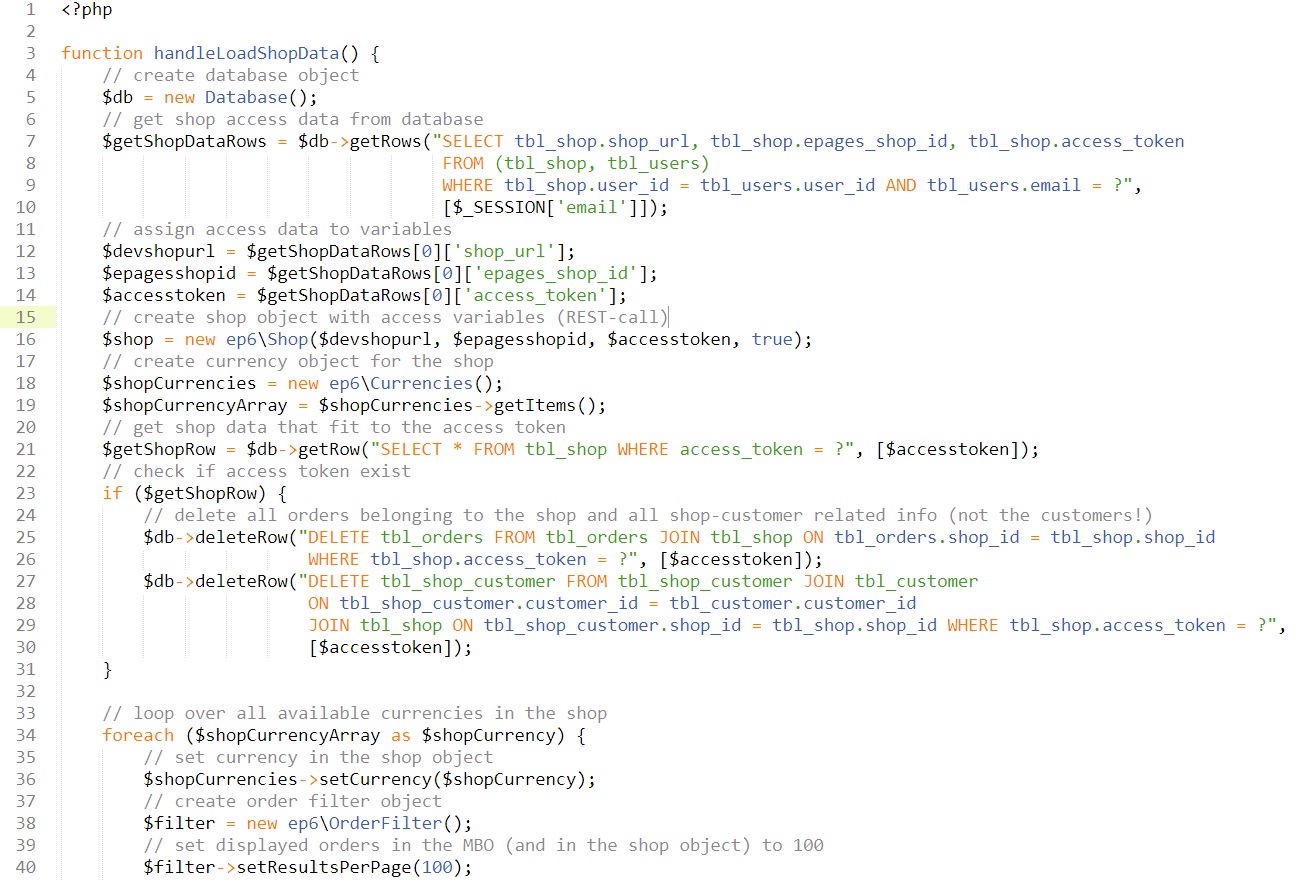
\includegraphics[page=1, width=1.0\textwidth]{shopphp1.png}
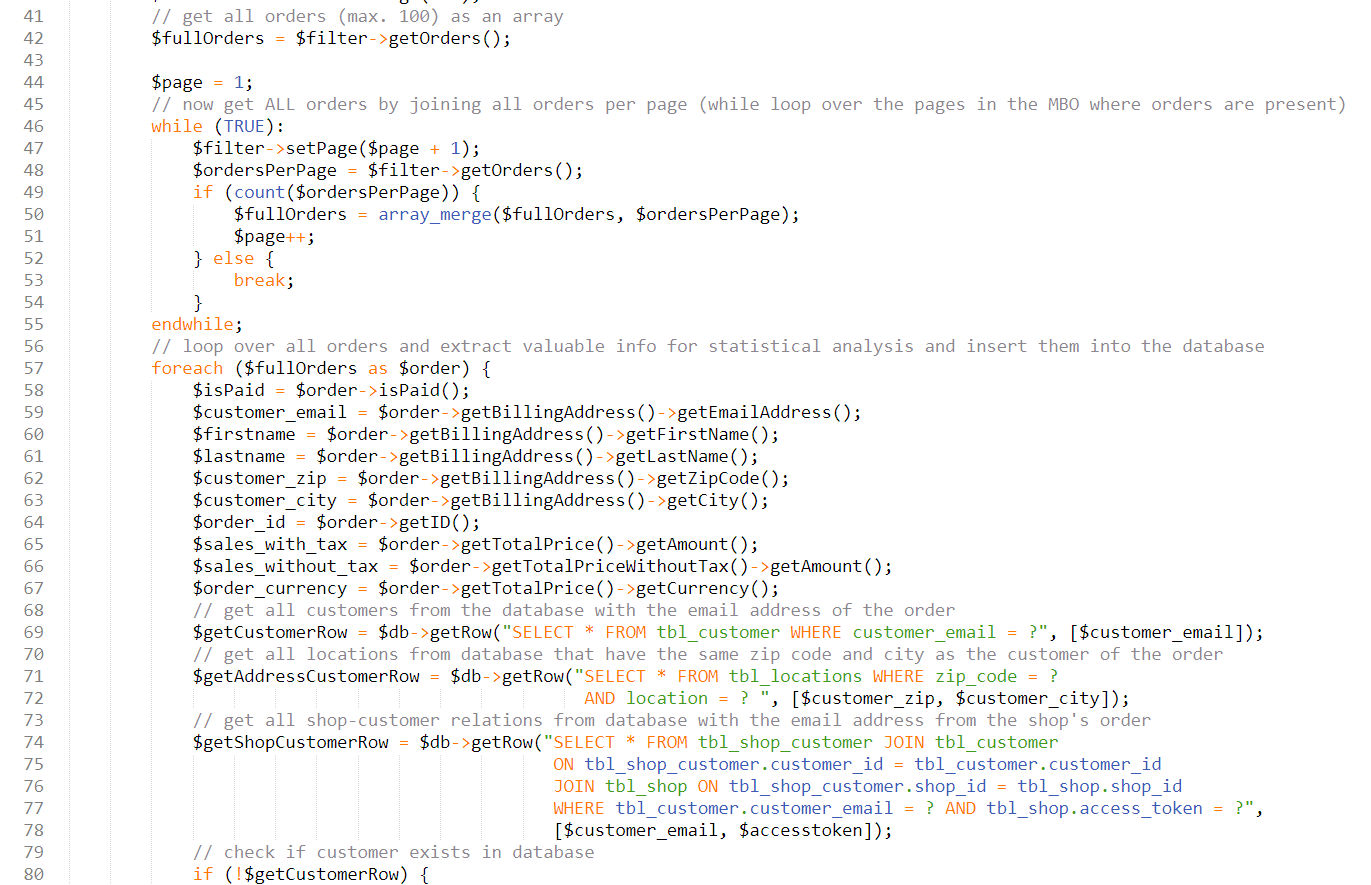
\includegraphics[page=1, width=1.0\textwidth]{shopphp2.png}
\end{center}
\begin{center}
\includegraphics[page=2, width=1.0\textwidth]{shopphp3.png}
\end{center}
\begin{center}
\includegraphics[page=2, width=1.0\textwidth]{shopphp4.png}
\end{center}



\end{document}
